% Options for packages loaded elsewhere
\PassOptionsToPackage{unicode}{hyperref}
\PassOptionsToPackage{hyphens}{url}
\documentclass[
]{article}
\usepackage{xcolor}
\usepackage[margin=1in]{geometry}
\usepackage{amsmath,amssymb}
\setcounter{secnumdepth}{5}
\usepackage{iftex}
\ifPDFTeX
  \usepackage[T1]{fontenc}
  \usepackage[utf8]{inputenc}
  \usepackage{textcomp} % provide euro and other symbols
\else % if luatex or xetex
  \usepackage{unicode-math} % this also loads fontspec
  \defaultfontfeatures{Scale=MatchLowercase}
  \defaultfontfeatures[\rmfamily]{Ligatures=TeX,Scale=1}
\fi
\usepackage{lmodern}
\ifPDFTeX\else
  % xetex/luatex font selection
\fi
% Use upquote if available, for straight quotes in verbatim environments
\IfFileExists{upquote.sty}{\usepackage{upquote}}{}
\IfFileExists{microtype.sty}{% use microtype if available
  \usepackage[]{microtype}
  \UseMicrotypeSet[protrusion]{basicmath} % disable protrusion for tt fonts
}{}
\makeatletter
\@ifundefined{KOMAClassName}{% if non-KOMA class
  \IfFileExists{parskip.sty}{%
    \usepackage{parskip}
  }{% else
    \setlength{\parindent}{0pt}
    \setlength{\parskip}{6pt plus 2pt minus 1pt}}
}{% if KOMA class
  \KOMAoptions{parskip=half}}
\makeatother
\usepackage{color}
\usepackage{fancyvrb}
\newcommand{\VerbBar}{|}
\newcommand{\VERB}{\Verb[commandchars=\\\{\}]}
\DefineVerbatimEnvironment{Highlighting}{Verbatim}{commandchars=\\\{\}}
% Add ',fontsize=\small' for more characters per line
\usepackage{framed}
\definecolor{shadecolor}{RGB}{248,248,248}
\newenvironment{Shaded}{\begin{snugshade}}{\end{snugshade}}
\newcommand{\AlertTok}[1]{\textcolor[rgb]{0.94,0.16,0.16}{#1}}
\newcommand{\AnnotationTok}[1]{\textcolor[rgb]{0.56,0.35,0.01}{\textbf{\textit{#1}}}}
\newcommand{\AttributeTok}[1]{\textcolor[rgb]{0.13,0.29,0.53}{#1}}
\newcommand{\BaseNTok}[1]{\textcolor[rgb]{0.00,0.00,0.81}{#1}}
\newcommand{\BuiltInTok}[1]{#1}
\newcommand{\CharTok}[1]{\textcolor[rgb]{0.31,0.60,0.02}{#1}}
\newcommand{\CommentTok}[1]{\textcolor[rgb]{0.56,0.35,0.01}{\textit{#1}}}
\newcommand{\CommentVarTok}[1]{\textcolor[rgb]{0.56,0.35,0.01}{\textbf{\textit{#1}}}}
\newcommand{\ConstantTok}[1]{\textcolor[rgb]{0.56,0.35,0.01}{#1}}
\newcommand{\ControlFlowTok}[1]{\textcolor[rgb]{0.13,0.29,0.53}{\textbf{#1}}}
\newcommand{\DataTypeTok}[1]{\textcolor[rgb]{0.13,0.29,0.53}{#1}}
\newcommand{\DecValTok}[1]{\textcolor[rgb]{0.00,0.00,0.81}{#1}}
\newcommand{\DocumentationTok}[1]{\textcolor[rgb]{0.56,0.35,0.01}{\textbf{\textit{#1}}}}
\newcommand{\ErrorTok}[1]{\textcolor[rgb]{0.64,0.00,0.00}{\textbf{#1}}}
\newcommand{\ExtensionTok}[1]{#1}
\newcommand{\FloatTok}[1]{\textcolor[rgb]{0.00,0.00,0.81}{#1}}
\newcommand{\FunctionTok}[1]{\textcolor[rgb]{0.13,0.29,0.53}{\textbf{#1}}}
\newcommand{\ImportTok}[1]{#1}
\newcommand{\InformationTok}[1]{\textcolor[rgb]{0.56,0.35,0.01}{\textbf{\textit{#1}}}}
\newcommand{\KeywordTok}[1]{\textcolor[rgb]{0.13,0.29,0.53}{\textbf{#1}}}
\newcommand{\NormalTok}[1]{#1}
\newcommand{\OperatorTok}[1]{\textcolor[rgb]{0.81,0.36,0.00}{\textbf{#1}}}
\newcommand{\OtherTok}[1]{\textcolor[rgb]{0.56,0.35,0.01}{#1}}
\newcommand{\PreprocessorTok}[1]{\textcolor[rgb]{0.56,0.35,0.01}{\textit{#1}}}
\newcommand{\RegionMarkerTok}[1]{#1}
\newcommand{\SpecialCharTok}[1]{\textcolor[rgb]{0.81,0.36,0.00}{\textbf{#1}}}
\newcommand{\SpecialStringTok}[1]{\textcolor[rgb]{0.31,0.60,0.02}{#1}}
\newcommand{\StringTok}[1]{\textcolor[rgb]{0.31,0.60,0.02}{#1}}
\newcommand{\VariableTok}[1]{\textcolor[rgb]{0.00,0.00,0.00}{#1}}
\newcommand{\VerbatimStringTok}[1]{\textcolor[rgb]{0.31,0.60,0.02}{#1}}
\newcommand{\WarningTok}[1]{\textcolor[rgb]{0.56,0.35,0.01}{\textbf{\textit{#1}}}}
\usepackage{longtable,booktabs,array}
\newcounter{none} % for unnumbered tables
\usepackage{calc} % for calculating minipage widths
% Correct order of tables after \paragraph or \subparagraph
\usepackage{etoolbox}
\makeatletter
\patchcmd\longtable{\par}{\if@noskipsec\mbox{}\fi\par}{}{}
\makeatother
% Allow footnotes in longtable head/foot
\IfFileExists{footnotehyper.sty}{\usepackage{footnotehyper}}{\usepackage{footnote}}
\makesavenoteenv{longtable}
\usepackage{graphicx}
\makeatletter
\newsavebox\pandoc@box
\newcommand*\pandocbounded[1]{% scales image to fit in text height/width
  \sbox\pandoc@box{#1}%
  \Gscale@div\@tempa{\textheight}{\dimexpr\ht\pandoc@box+\dp\pandoc@box\relax}%
  \Gscale@div\@tempb{\linewidth}{\wd\pandoc@box}%
  \ifdim\@tempb\p@<\@tempa\p@\let\@tempa\@tempb\fi% select the smaller of both
  \ifdim\@tempa\p@<\p@\scalebox{\@tempa}{\usebox\pandoc@box}%
  \else\usebox{\pandoc@box}%
  \fi%
}
% Set default figure placement to htbp
\def\fps@figure{htbp}
\makeatother
\setlength{\emergencystretch}{3em} % prevent overfull lines
\providecommand{\tightlist}{%
  \setlength{\itemsep}{0pt}\setlength{\parskip}{0pt}}
\usepackage{bookmark}
\IfFileExists{xurl.sty}{\usepackage{xurl}}{} % add URL line breaks if available
\urlstyle{same}
\hypersetup{
  pdftitle={Multistage variance estimation with qvar\_ms},
  pdfauthor={Thomas Delclite},
  hidelinks,
  pdfcreator={LaTeX via pandoc}}

\title{Multistage variance estimation with qvar\_ms}
\author{Thomas Delclite}
\date{2026-09-01}

\begin{document}
\maketitle

{
\setcounter{tocdepth}{2}
\tableofcontents
}
\section{Introduction}\label{introduction}

The \texttt{qvar()} function performs analytical variance estimation in
the most common single-stage case: stratified simple random sampling,
non-response correction through reweighting, calibration on margins.
\texttt{qvar\_ms()} extends this logic to \textbf{multistage designs}:
units of stage 2 are drawn within the units of stage 1, units of stage 3
within the units of stage 2, and so on, with non-response correction
possibly occurring at each stage and calibration at one given stage.

The variance is estimated as the sum of the conditional variances of
each stage, following the Rao (1975) formula as implemented in the SAS
Poulpe macros (Caron, 1998) and natively supported by the variance
functions of the gustave package: at each stage, the variance
contributions (\texttt{var\_srs()}, \texttt{var\_pois()}) are
\emph{linearly} weighted by the cumulated corrected weight of the stages
above, through their \texttt{w} argument, and the first-stage variance
is computed on the estimated totals per primary sampling unit.

This vignette walks through \textbf{nine cases of increasing
complexity}, using the simulated Labour Force Survey (LFS) data shipped
with the package (\texttt{lfs\_samp\_area}: areas, i.e.~primary sampling
units; \texttt{lfs\_samp\_dwel}: dwellings sampled within areas;
\texttt{lfs\_samp\_ind}: individuals within dwellings).

\begin{Shaded}
\begin{Highlighting}[]
\FunctionTok{library}\NormalTok{(gustave)}
\FunctionTok{library}\NormalTok{(dplyr)}
\FunctionTok{library}\NormalTok{(purrr)}

\NormalTok{lfs\_samp\_area }\OtherTok{\textless{}{-}}\NormalTok{ gustave}\SpecialCharTok{::}\NormalTok{lfs\_samp\_area}
\NormalTok{lfs\_samp\_dwel }\OtherTok{\textless{}{-}}\NormalTok{ gustave}\SpecialCharTok{::}\NormalTok{lfs\_samp\_dwel}
\NormalTok{lfs\_samp\_ind  }\OtherTok{\textless{}{-}}\NormalTok{ gustave}\SpecialCharTok{::}\NormalTok{lfs\_samp\_ind}
\end{Highlighting}
\end{Shaded}

\section{\texorpdfstring{How to use
\texttt{qvar\_ms()}}{How to use qvar\_ms()}}\label{how-to-use-qvar_ms}

The best way to learn \texttt{qvar\_ms()} is to build wrappers of
increasing complexity. This section walks through nine cases, each
introducing exactly one new feature of the interface: from a
single-stage design that reproduces \texttt{qvar()} (case 1), through
two-stage designs with non-response correction, stratification and
calibration (cases 2 to 6), to three-stage designs with corrections at
several stages and calibration at an intermediate stage (cases 7 to 9).

The cases are cumulative --- the data prepared in one case is reused in
the next --- and follow a fixed pattern: the \texttt{qvar\_ms()} call
first, then a hand-built equivalent using
\texttt{define\_variance\_wrapper()} and the core \texttt{gustave}
functions, which makes every methodological step explicit and serves as
ground truth. Readers in a hurry can jump to the case matching their
design and work backwards.

\texttt{qvar\_ms()} uses \texttt{varDT()} to estimate the variance of
the estimator of a total in the case of a balanced sampling design with
equal or unequal probabilities using Deville-Tillé (2005) formula. All
examples use the function \texttt{var\_srs()}, which is a convenience
wrapper for the (stratified) simple random sampling case.

\subsection{Conventions}\label{conventions}

Before anything else, the conventions used by \texttt{qvar\_ms()} ---
most errors in practice come from overlooking one of them:

\begin{itemize}
\tightlist
\item
  \textbf{Stage ordering.} Stage 1 is the highest sampling stage
  (e.g.~primary sampling units); stage \texttt{L\ =\ sampling\_stages}
  is the final stage (surveyed units). \texttt{data} is a list of
  \texttt{L} data.frames ordered from stage 1 to stage \texttt{L}, each
  containing \textbf{all} the units sampled at the corresponding stage,
  including out-of-scope and non-responding units.
\item
  \textbf{Parent linkage.} Each file from stage 2 onwards contains a
  variable identifying the unit of the stage above (\texttt{parent\_id}
  argument; by default, the \texttt{id} variable of the previous stage
  is assumed to be present).
\item
  \textbf{Conditional weights.} \texttt{sampling\_weight} and
  \texttt{nrc\_weight} are \textbf{conditional} weights at the
  considered stage: the inverse of the inclusion (resp. response)
  probability \emph{given the stages above}. This is the single most
  important convention of the interface.
\item
  \textbf{Response probability.} \texttt{response\_prob} can be used
  instead of \texttt{nrc\_weight} to include response probability at
  each stage of non-response.
\item
  \textbf{Cumulated calibration weight.} \texttt{calibration\_weight} is
  the \textbf{cumulated} weight at the calibration stage --- the weight
  actually used in the calibration equations.
\item
  \textbf{Last stage only.} \texttt{dissemination\_dummy},
  \texttt{dissemination\_weight} and \texttt{scope\_dummy} refer to the
  last stage file.
\item
  \textbf{Per-stage arguments.} Non-response correction may be declared
  at each stage through list-valued arguments (\texttt{nrc\_weight},
  \texttt{response\_dummy}, \texttt{nrc\_dummy}); a single variable name
  is assigned to the last stage. Calibration is declared at one single
  stage (\texttt{calibration\_stage}, last stage by default).
\end{itemize}

{\def\LTcaptype{none} % do not increment counter
\begin{longtable}[]{@{}
  >{\raggedright\arraybackslash}p{(\linewidth - 6\tabcolsep) * \real{0.2892}}
  >{\raggedright\arraybackslash}p{(\linewidth - 6\tabcolsep) * \real{0.2410}}
  >{\raggedright\arraybackslash}p{(\linewidth - 6\tabcolsep) * \real{0.2289}}
  >{\raggedright\arraybackslash}p{(\linewidth - 6\tabcolsep) * \real{0.2410}}@{}}
\toprule\noalign{}
\begin{minipage}[b]{\linewidth}\raggedright
Argument
\end{minipage} & \begin{minipage}[b]{\linewidth}\raggedright
Per stage?
\end{minipage} & \begin{minipage}[b]{\linewidth}\raggedright
Weight convention
\end{minipage} & \begin{minipage}[b]{\linewidth}\raggedright
Default
\end{minipage} \\
\midrule\noalign{}
\endhead
\bottomrule\noalign{}
\endlastfoot
\texttt{id} & yes (length L) & --- & required \\
\texttt{parent\_id} & stages 2..L & --- & id of stage above \\
\texttt{sampling\_weight} & yes (length L) & conditional & required \\
\texttt{strata} & yes (list) & --- & none \\
\texttt{nrc\_weight}, \texttt{response\_dummy},
\texttt{response\_dummy}, \texttt{nrc\_dummy} & yes (list) & conditional
& last stage \\
\texttt{calibration\_stage} & one stage & --- & last stage \\
\texttt{calibration\_weight} & one stage & \textbf{cumulated} & none \\
\texttt{dissemination\_*}, \texttt{scope\_dummy} & last stage &
cumulated & required / none \\
\end{longtable}
}

\subsection{\texorpdfstring{Case 1: single stage --- backward
compatibility with
\texttt{qvar()}}{Case 1: single stage --- backward compatibility with qvar()}}\label{case-1-single-stage-backward-compatibility-with-qvar}

When \texttt{data} is a single data.frame (or
\texttt{sampling\_stages\ =\ 1}), \texttt{qvar\_ms()} degenerates to the
standard single-stage case and should reproduce \texttt{qvar()} exactly.
This is the first thing to check.

\begin{Shaded}
\begin{Highlighting}[]
\NormalTok{lfs\_samp\_dwel}\SpecialCharTok{$}\NormalTok{diss    }\OtherTok{\textless{}{-}} \ConstantTok{TRUE}
\NormalTok{lfs\_samp\_dwel}\SpecialCharTok{$}\NormalTok{w\_dwel  }\OtherTok{\textless{}{-}} \DecValTok{1} \SpecialCharTok{/}\NormalTok{ lfs\_samp\_dwel}\SpecialCharTok{$}\NormalTok{pik\_dwel}
\NormalTok{lfs\_samp\_dwel}\SpecialCharTok{$}\NormalTok{w\_final }\OtherTok{\textless{}{-}} \DecValTok{1} \SpecialCharTok{/}\NormalTok{ lfs\_samp\_dwel}\SpecialCharTok{$}\NormalTok{pik}
\end{Highlighting}
\end{Shaded}

\begin{Shaded}
\begin{Highlighting}[]
\NormalTok{qvar1 }\OtherTok{\textless{}{-}} \FunctionTok{qvar\_ms}\NormalTok{(}
  \AttributeTok{data =}\NormalTok{ lfs\_samp\_dwel,}
  \AttributeTok{id =} \StringTok{"id\_dwel"}\NormalTok{,}
  \AttributeTok{dissemination\_dummy =} \StringTok{"diss"}\NormalTok{,}
  \AttributeTok{dissemination\_weight =} \StringTok{"w\_final"}\NormalTok{,}
  \AttributeTok{sampling\_weight =} \StringTok{"w\_final"}\NormalTok{,}
  \AttributeTok{define =} \ConstantTok{TRUE}
\NormalTok{)}
\CommentTok{\#\textgreater{} Survey variance estimation with the gustave package}
\CommentTok{\#\textgreater{} }
\CommentTok{\#\textgreater{} The following features are taken into account:}
\CommentTok{\#\textgreater{}   {-} simple random sampling WITHOUT stratification}
\CommentTok{\#\textgreater{} Note: As define = TRUE, a ready{-}to{-}use variance wrapper is (invisibly) returned.}

\NormalTok{qvar1b }\OtherTok{\textless{}{-}} \FunctionTok{qvar}\NormalTok{(}
  \AttributeTok{data =}\NormalTok{ lfs\_samp\_dwel,}
  \AttributeTok{id =} \StringTok{"id\_dwel"}\NormalTok{,}
  \AttributeTok{dissemination\_dummy =} \StringTok{"diss"}\NormalTok{,}
  \AttributeTok{dissemination\_weight =} \StringTok{"w\_final"}\NormalTok{,}
  \AttributeTok{sampling\_weight =} \StringTok{"w\_final"}\NormalTok{,}
  \AttributeTok{define =} \ConstantTok{TRUE}
\NormalTok{)}
\CommentTok{\#\textgreater{} Survey variance estimation with the gustave package}
\CommentTok{\#\textgreater{} }
\CommentTok{\#\textgreater{} The following features are taken into account:}
\CommentTok{\#\textgreater{}   {-} simple random sampling WITHOUT stratification}
\CommentTok{\#\textgreater{} }
\CommentTok{\#\textgreater{} Note: As define = TRUE, a ready{-}to{-}use variance wrapper is (invisibly) returned.}

\FunctionTok{qvar1}\NormalTok{(lfs\_samp\_dwel, }\FunctionTok{total}\NormalTok{(income))}
\CommentTok{\#\textgreater{}                call  n      est  variance      std       cv  lower    upper}
\CommentTok{\#\textgreater{} 1 total(y = income) 80 198417.3 136946649 11702.42 5.897882 175481 221353.7}
\FunctionTok{qvar1b}\NormalTok{(lfs\_samp\_dwel, }\FunctionTok{total}\NormalTok{(income))}
\CommentTok{\#\textgreater{}                call  n      est  variance      std       cv  lower    upper}
\CommentTok{\#\textgreater{} 1 total(y = income) 80 198417.3 136946649 11702.42 5.897882 175481 221353.7}
\end{Highlighting}
\end{Shaded}

Both wrappers return the same estimate and the same variance: with one
stage, the cumulated weight of the ``stages above'' is 1 everywhere and
the Rao weighting is inactive.

\subsection{Case 2: two-stage design, no non-response, no
calibration}\label{case-2-two-stage-design-no-non-response-no-calibration}

We now use the area file as a first stage. For this introductory case
the area weights are made equal (no stratification at stage 1), as
\texttt{qvar\_ms()} --- like \texttt{qvar()} --- relies on the simple
random sampling formula within strata and would otherwise warn and use
the mean weight per stratum. The final dwelling weight is rebuilt as the
product of the \textbf{conditional} weights of the two stages.

\begin{Shaded}
\begin{Highlighting}[]
\NormalTok{lfs\_samp\_area}\SpecialCharTok{$}\NormalTok{w\_area }\OtherTok{\textless{}{-}}\NormalTok{ base}\SpecialCharTok{::}\FunctionTok{mean}\NormalTok{(}\DecValTok{1} \SpecialCharTok{/}\NormalTok{ lfs\_samp\_area}\SpecialCharTok{$}\NormalTok{pik\_area)}

\NormalTok{lfs\_samp\_dwel }\OtherTok{\textless{}{-}}\NormalTok{ lfs\_samp\_dwel }\SpecialCharTok{\%\textgreater{}\%}
  \FunctionTok{left\_join}\NormalTok{(lfs\_samp\_area }\SpecialCharTok{\%\textgreater{}\%} \FunctionTok{select}\NormalTok{(id\_area, w\_area), }\AttributeTok{by =} \StringTok{"id\_area"}\NormalTok{)}

\NormalTok{lfs\_samp\_dwel}\SpecialCharTok{$}\NormalTok{w\_dwel  }\OtherTok{\textless{}{-}} \DecValTok{1} \SpecialCharTok{/}\NormalTok{ lfs\_samp\_dwel}\SpecialCharTok{$}\NormalTok{pik\_dwel}
\NormalTok{lfs\_samp\_dwel}\SpecialCharTok{$}\NormalTok{w\_final }\OtherTok{\textless{}{-}}\NormalTok{ lfs\_samp\_dwel}\SpecialCharTok{$}\NormalTok{w\_dwel }\SpecialCharTok{*}\NormalTok{ lfs\_samp\_dwel}\SpecialCharTok{$}\NormalTok{w\_area}
\end{Highlighting}
\end{Shaded}

\begin{Shaded}
\begin{Highlighting}[]
\NormalTok{qvar2 }\OtherTok{\textless{}{-}} \FunctionTok{qvar\_ms}\NormalTok{(}
  \CommentTok{\# One file per stage, from the highest to the lowest}
  \AttributeTok{data =} \FunctionTok{list}\NormalTok{(lfs\_samp\_area, lfs\_samp\_dwel),}
  \AttributeTok{sampling\_stages =} \DecValTok{2}\NormalTok{,}
  \AttributeTok{id =} \FunctionTok{c}\NormalTok{(}\StringTok{"id\_area"}\NormalTok{, }\StringTok{"id\_dwel"}\NormalTok{),}
  \AttributeTok{parent\_id =} \FunctionTok{c}\NormalTok{(}\StringTok{"id\_area"}\NormalTok{),}
  \AttributeTok{dissemination\_dummy =} \StringTok{"diss"}\NormalTok{,}
  \AttributeTok{dissemination\_weight =} \StringTok{"w\_final"}\NormalTok{,}
  \CommentTok{\# Conditional sampling weights, one per stage}
  \AttributeTok{sampling\_weight =} \FunctionTok{c}\NormalTok{(}\StringTok{"w\_area"}\NormalTok{, }\StringTok{"w\_dwel"}\NormalTok{),}
  \AttributeTok{define =} \ConstantTok{TRUE}
\NormalTok{)}
\CommentTok{\#\textgreater{} Survey variance estimation with the gustave package}
\CommentTok{\#\textgreater{} }
\CommentTok{\#\textgreater{} The following features are taken into account:}
\CommentTok{\#\textgreater{}   {-} 2{-}stage sampling design}
\CommentTok{\#\textgreater{}   {-} stage 1: simple random sampling WITHOUT stratification}
\CommentTok{\#\textgreater{}   {-} stage 2: simple random sampling WITHOUT stratification (within the units of the stage above)}
\CommentTok{\#\textgreater{} Note: At stage 2, units are drawn within the units of the stage above: the effective strata used for variance estimation are the crossing of the parent unit (id\_area).}
\CommentTok{\#\textgreater{} Note: As define = TRUE, a ready{-}to{-}use variance wrapper is (invisibly) returned.}
\end{Highlighting}
\end{Shaded}

The hand-built equivalent makes the Rao (1975) decomposition explicit:
one within-area variance per primary unit, multiplied by the area weight
(\emph{first power} --- this is the Rao row weight), plus the
first-stage variance computed on the estimated area totals. The
generalization to more stages and to non-response phases proceeds
recursively, the Rao row weight at stage \(k\) being the cumulated
corrected weight of stages \(1, \dots, k-1\). This is the estimator
implemented by the SAS \texttt{Poulpe} macros (Caron, 1998).

\begin{Shaded}
\begin{Highlighting}[]
\NormalTok{var\_srs\_two }\OtherTok{\textless{}{-}} \ControlFlowTok{function}\NormalTok{(y, smp\_area, smp\_dwel) \{}

\NormalTok{  variance }\OtherTok{\textless{}{-}} \FunctionTok{list}\NormalTok{()}
\NormalTok{  y }\OtherTok{\textless{}{-}} \FunctionTok{add\_zero}\NormalTok{(y, }\AttributeTok{rownames =}\NormalTok{ smp\_dwel}\SpecialCharTok{$}\NormalTok{id\_dwel)}

  \CommentTok{\# Stage 2: one SRS variance per area, weighted by the area weight}
\NormalTok{  variance[[}\StringTok{"srs{-}dwel"}\NormalTok{]] }\OtherTok{\textless{}{-}} \FunctionTok{unique}\NormalTok{(smp\_dwel}\SpecialCharTok{$}\NormalTok{id\_area) }\SpecialCharTok{\%\textgreater{}\%} \FunctionTok{map}\NormalTok{(}\SpecialCharTok{\textasciitilde{}}\NormalTok{\{}
\NormalTok{    sub }\OtherTok{\textless{}{-}}\NormalTok{ smp\_dwel }\SpecialCharTok{\%\textgreater{}\%} \FunctionTok{filter}\NormalTok{(id\_area }\SpecialCharTok{==}\NormalTok{ .x)}
\NormalTok{    w\_area }\OtherTok{\textless{}{-}} \FunctionTok{unique}\NormalTok{(sub}\SpecialCharTok{$}\NormalTok{w\_area)}
    \FunctionTok{var\_srs}\NormalTok{(}
\NormalTok{      y[sub}\SpecialCharTok{$}\NormalTok{id\_dwel, , }\AttributeTok{drop =} \ConstantTok{FALSE}\NormalTok{],}
      \AttributeTok{pik =}\NormalTok{ sub}\SpecialCharTok{$}\NormalTok{pik\_dwel}
\NormalTok{    ) }\SpecialCharTok{*}\NormalTok{ w\_area}
\NormalTok{  \}) }\SpecialCharTok{\%\textgreater{}\%}\NormalTok{ unlist }\SpecialCharTok{\%\textgreater{}\%}\NormalTok{ sum}

  \CommentTok{\# Aggregation: estimated totals per area}
\NormalTok{  y\_area }\OtherTok{\textless{}{-}} \FunctionTok{sum\_by}\NormalTok{(y, }\AttributeTok{by =}\NormalTok{ smp\_dwel}\SpecialCharTok{$}\NormalTok{id\_area, }\AttributeTok{w =} \DecValTok{1} \SpecialCharTok{/}\NormalTok{ smp\_dwel}\SpecialCharTok{$}\NormalTok{pik\_dwel)}

  \CommentTok{\# Stage 1: SRS variance on the estimated area totals}
\NormalTok{  variance[[}\StringTok{"srs{-}area"}\NormalTok{]] }\OtherTok{\textless{}{-}} \FunctionTok{var\_srs}\NormalTok{(}
\NormalTok{    y\_area[smp\_area}\SpecialCharTok{$}\NormalTok{id\_area, , }\AttributeTok{drop =} \ConstantTok{FALSE}\NormalTok{], }
    \AttributeTok{pik =} \DecValTok{1} \SpecialCharTok{/}\NormalTok{ smp\_area}\SpecialCharTok{$}\NormalTok{w\_area}
\NormalTok{  )}

  \FunctionTok{print}\NormalTok{(}\FunctionTok{as.data.frame}\NormalTok{(variance))}
  \FunctionTok{Reduce}\NormalTok{(}\StringTok{\textasciigrave{}}\AttributeTok{+}\StringTok{\textasciigrave{}}\NormalTok{, variance)}
\NormalTok{\}}

\NormalTok{qvar2b }\OtherTok{\textless{}{-}} \FunctionTok{define\_variance\_wrapper}\NormalTok{(}
  \AttributeTok{variance\_function =}\NormalTok{ var\_srs\_two,}
  \AttributeTok{technical\_data    =} \FunctionTok{list}\NormalTok{(}\AttributeTok{smp\_area =}\NormalTok{ lfs\_samp\_area, }\AttributeTok{smp\_dwel =}\NormalTok{ lfs\_samp\_dwel),}
  \AttributeTok{reference\_id      =}\NormalTok{ lfs\_samp\_dwel}\SpecialCharTok{$}\NormalTok{id\_dwel,}
  \AttributeTok{reference\_weight  =}\NormalTok{ lfs\_samp\_dwel}\SpecialCharTok{$}\NormalTok{w\_final,}
  \AttributeTok{default\_id        =} \StringTok{"id\_dwel"}
\NormalTok{)}

\FunctionTok{qvar2}\NormalTok{(lfs\_samp\_dwel, }\FunctionTok{total}\NormalTok{(income))}
\CommentTok{\#\textgreater{}                call  n      est  variance      std      cv    lower    upper}
\CommentTok{\#\textgreater{} 1 total(y = income) 80 198343.6 523055781 22870.41 11.5307 153518.4 243168.8}
\FunctionTok{qvar2b}\NormalTok{(lfs\_samp\_dwel, }\FunctionTok{total}\NormalTok{(income))}
\CommentTok{\#\textgreater{}   srs.dwel  srs.area}
\CommentTok{\#\textgreater{} 1  5096232 517959549}
\CommentTok{\#\textgreater{}                call  n      est  variance      std      cv    lower    upper}
\CommentTok{\#\textgreater{} 1 total(y = income) 80 198343.6 523055781 22870.41 11.5307 153518.4 243168.8}
\end{Highlighting}
\end{Shaded}

Note how \texttt{qvar\_ms()} achieves the per-area computation: at stage
2, the effective strata are the crossing of the parent unit and of the
declared strata variable (here, none), so that one single stratified
\texttt{var\_srs()} call is algebraically identical to the sum of
per-area variances --- the Rao weight, constant within each area, being
passed through the \texttt{w} argument. The components printed by the
hand-built version (\texttt{srs-dwel}, \texttt{srs-area}) correspond
one-to-one to the sampling\_stage2 and sampling\_stage1 components that
\texttt{qvar\_ms()} reports in its ``components'' diagnostic (see
diagnostic section below):

\begin{Shaded}
\begin{Highlighting}[]
\FunctionTok{qvar2}\NormalTok{(lfs\_samp\_dwel, }\FunctionTok{total}\NormalTok{(income), }\AttributeTok{diagnostics =} \StringTok{"components"}\NormalTok{)}
\CommentTok{\#\textgreater{} }
\CommentTok{\#\textgreater{} {-}{-} Variance components {-}{-}}
\CommentTok{\#\textgreater{}   sampling\_stage2     5.096e+06    1.0 \%  }
\CommentTok{\#\textgreater{}   sampling\_stage1      5.18e+08   99.0 \%  \#\#\#\#\#\#\#\#\#\#\#\#\#\#\#\#\#\#\#\#}
\CommentTok{\#\textgreater{}   TOTAL               5.231e+08}
\CommentTok{\#\textgreater{}                call  n      est  variance      std      cv    lower    upper}
\CommentTok{\#\textgreater{} 1 total(y = income) 80 198343.6 523055781 22870.41 11.5307 153518.4 243168.8}
\end{Highlighting}
\end{Shaded}

\subsection{Case 3: non-response correction at the last
stage}\label{case-3-non-response-correction-at-the-last-stage}

We simulate a response mechanism at the dwelling stage. \textbf{The
non-response correction weight passed to \texttt{qvar\_ms()} must be
conditional to the current stage}: \texttt{w\_nrc\ =\ w\_dwel\ /\ prep},
not \texttt{w\_final\ /\ prep}. Passing a cumulated weight here is the
most common mistake --- it silently deflates the response probabilities
computed internally (\texttt{sampling\_weight\ /\ nrc\_weight}) and
propagates a spurious factor to every stage of the decomposition. A
safer alternative is to pass the estimated response probabilities
directly, through the \texttt{response\_prob} argument: probabilities
have no cumulated counterpart, so this mistake simply cannot occur. The
two arguments are mutually exclusive --- declare one or the other at
each corrected stage, not both.

\begin{Shaded}
\begin{Highlighting}[]
\FunctionTok{set.seed}\NormalTok{(}\DecValTok{123}\NormalTok{)}
\NormalTok{lfs\_samp\_dwel}\SpecialCharTok{$}\NormalTok{rand  }\OtherTok{\textless{}{-}} \FunctionTok{runif}\NormalTok{(}\FunctionTok{nrow}\NormalTok{(lfs\_samp\_dwel))}
\NormalTok{lfs\_samp\_dwel}\SpecialCharTok{$}\NormalTok{rep   }\OtherTok{\textless{}{-}}\NormalTok{ lfs\_samp\_dwel}\SpecialCharTok{$}\NormalTok{rand }\SpecialCharTok{\textless{}=} \FloatTok{0.6}
\NormalTok{lfs\_samp\_dwel}\SpecialCharTok{$}\NormalTok{prep   }\OtherTok{\textless{}{-}} \FloatTok{0.6}
\NormalTok{lfs\_samp\_dwel}\SpecialCharTok{$}\NormalTok{w\_nrc }\OtherTok{\textless{}{-}}\NormalTok{ lfs\_samp\_dwel}\SpecialCharTok{$}\NormalTok{w\_dwel }\SpecialCharTok{/}\NormalTok{ lfs\_samp\_dwel}\SpecialCharTok{$}\NormalTok{prep   }\CommentTok{\# conditional!}
\NormalTok{lfs\_samp\_dwel}\SpecialCharTok{$}\NormalTok{w\_final }\OtherTok{\textless{}{-}}\NormalTok{ lfs\_samp\_dwel}\SpecialCharTok{$}\NormalTok{w\_nrc }\SpecialCharTok{*}\NormalTok{ lfs\_samp\_dwel}\SpecialCharTok{$}\NormalTok{w\_area}
\NormalTok{lfs\_samp\_dwel}\SpecialCharTok{$}\NormalTok{w\_final[}\SpecialCharTok{!}\NormalTok{lfs\_samp\_dwel}\SpecialCharTok{$}\NormalTok{rep] }\OtherTok{\textless{}{-}} \DecValTok{0}
\NormalTok{lfs\_samp\_dwel}\SpecialCharTok{$}\NormalTok{income[}\SpecialCharTok{!}\NormalTok{lfs\_samp\_dwel}\SpecialCharTok{$}\NormalTok{rep]  }\OtherTok{\textless{}{-}} \DecValTok{0}
\end{Highlighting}
\end{Shaded}

\begin{Shaded}
\begin{Highlighting}[]
\NormalTok{qvar3 }\OtherTok{\textless{}{-}} \FunctionTok{qvar\_ms}\NormalTok{(}
  \AttributeTok{data =} \FunctionTok{list}\NormalTok{(lfs\_samp\_area, lfs\_samp\_dwel),}
  \AttributeTok{sampling\_stages =} \DecValTok{2}\NormalTok{,}
  \AttributeTok{id =} \FunctionTok{c}\NormalTok{(}\StringTok{"id\_area"}\NormalTok{, }\StringTok{"id\_dwel"}\NormalTok{),}
  \AttributeTok{parent\_id =} \FunctionTok{c}\NormalTok{(}\StringTok{"id\_area"}\NormalTok{),}
  \AttributeTok{dissemination\_dummy =} \StringTok{"rep"}\NormalTok{,}
  \AttributeTok{dissemination\_weight =} \StringTok{"w\_final"}\NormalTok{,}
  \AttributeTok{sampling\_weight =} \FunctionTok{c}\NormalTok{(}\StringTok{"w\_area"}\NormalTok{, }\StringTok{"w\_dwel"}\NormalTok{),}
  \CommentTok{\# Single names: assigned to the last stage by default}
  \AttributeTok{nrc\_weight =} \StringTok{"w\_nrc"}\NormalTok{,}
  \CommentTok{\# response\_prob = "prep", \# instead of nrc\_weight}
  \AttributeTok{response\_dummy =} \StringTok{"rep"}\NormalTok{,}
  \AttributeTok{define =} \ConstantTok{TRUE}
\NormalTok{)}
\CommentTok{\#\textgreater{} Note: The nrc\_weight argument is of length 1: it is assumed to refer to the last sampling stage (stage 2).}
\CommentTok{\#\textgreater{} Note: The response\_dummy argument is of length 1: it is assumed to refer to the last sampling stage (stage 2).}
\CommentTok{\#\textgreater{} Survey variance estimation with the gustave package}
\CommentTok{\#\textgreater{} }
\CommentTok{\#\textgreater{} The following features are taken into account:}
\CommentTok{\#\textgreater{}   {-} 2{-}stage sampling design}
\CommentTok{\#\textgreater{}   {-} stage 1: simple random sampling WITHOUT stratification}
\CommentTok{\#\textgreater{}   {-} stage 2: simple random sampling WITHOUT stratification (within the units of the stage above), with non{-}response correction through reweighting}
\CommentTok{\#\textgreater{} Note: At stage 2, units are drawn within the units of the stage above: the effective strata used for variance estimation are the crossing of the parent unit (id\_area).}
\CommentTok{\#\textgreater{} Note: As define = TRUE, a ready{-}to{-}use variance wrapper is (invisibly) returned.}
\end{Highlighting}
\end{Shaded}

In the hand-built version, the non-response variance is a Poisson term
whose Rao row weight is the cumulated design weight down to the current
stage (\texttt{w\_dwel\ *\ w\_area}), and the interest variable is
expanded by the inverse response probability before moving up:

\begin{Shaded}
\begin{Highlighting}[]
\NormalTok{var\_srs\_two }\OtherTok{\textless{}{-}} \ControlFlowTok{function}\NormalTok{(y, smp\_area, smp\_dwel) \{}

\NormalTok{  variance }\OtherTok{\textless{}{-}} \FunctionTok{list}\NormalTok{()}
\NormalTok{  resp\_dwel }\OtherTok{\textless{}{-}}\NormalTok{ smp\_dwel }\SpecialCharTok{\%\textgreater{}\%} \FunctionTok{filter}\NormalTok{(rep }\SpecialCharTok{==} \DecValTok{1}\NormalTok{)}

  \CommentTok{\# Non{-}response variance (Poisson, respondents only)}
\NormalTok{  variance[[}\StringTok{"nr"}\NormalTok{]] }\OtherTok{\textless{}{-}} \FunctionTok{var\_pois}\NormalTok{(}
\NormalTok{    y[resp\_dwel}\SpecialCharTok{$}\NormalTok{id\_dwel, , }\AttributeTok{drop =} \ConstantTok{FALSE}\NormalTok{],}
    \AttributeTok{pik =}\NormalTok{ resp\_dwel}\SpecialCharTok{$}\NormalTok{prep,}
    \AttributeTok{w   =}\NormalTok{ resp\_dwel}\SpecialCharTok{$}\NormalTok{w\_dwel }\SpecialCharTok{*}\NormalTok{ resp\_dwel}\SpecialCharTok{$}\NormalTok{w\_area}
\NormalTok{  )}

  \CommentTok{\# Reintroduce non{-}responding dwellings with zeros}
\NormalTok{  y }\OtherTok{\textless{}{-}} \FunctionTok{add\_zero}\NormalTok{(y, }\AttributeTok{rownames =}\NormalTok{ smp\_dwel}\SpecialCharTok{$}\NormalTok{id\_dwel)}

  \CommentTok{\# Stage 2 sampling variance on the NR{-}expanded variable, over ALL}
  \CommentTok{\# sampled dwellings (non{-}respondents count as zeros)}
\NormalTok{  variance[[}\StringTok{"srs{-}dwel"}\NormalTok{]] }\OtherTok{\textless{}{-}} \FunctionTok{unique}\NormalTok{(smp\_dwel}\SpecialCharTok{$}\NormalTok{id\_area) }\SpecialCharTok{\%\textgreater{}\%} \FunctionTok{map}\NormalTok{(}\SpecialCharTok{\textasciitilde{}}\NormalTok{\{}
\NormalTok{    sub }\OtherTok{\textless{}{-}}\NormalTok{ smp\_dwel }\SpecialCharTok{\%\textgreater{}\%} \FunctionTok{filter}\NormalTok{(id\_area }\SpecialCharTok{==}\NormalTok{ .x)}
\NormalTok{    w\_area }\OtherTok{\textless{}{-}} \FunctionTok{unique}\NormalTok{(sub}\SpecialCharTok{$}\NormalTok{w\_area)}
    \FunctionTok{var\_srs}\NormalTok{(}
\NormalTok{      y[sub}\SpecialCharTok{$}\NormalTok{id\_dwel, , }\AttributeTok{drop =} \ConstantTok{FALSE}\NormalTok{] }\SpecialCharTok{/}\NormalTok{ sub}\SpecialCharTok{$}\NormalTok{prep,}
      \AttributeTok{pik =}\NormalTok{ sub}\SpecialCharTok{$}\NormalTok{pik\_dwel}
\NormalTok{    ) }\SpecialCharTok{*}\NormalTok{ w\_area}
\NormalTok{  \}) }\SpecialCharTok{\%\textgreater{}\%}\NormalTok{ unlist }\SpecialCharTok{\%\textgreater{}\%}\NormalTok{ sum}

\NormalTok{  y\_area }\OtherTok{\textless{}{-}} \FunctionTok{sum\_by}\NormalTok{(y }\SpecialCharTok{/}\NormalTok{ smp\_dwel}\SpecialCharTok{$}\NormalTok{prep, }\AttributeTok{by =}\NormalTok{ smp\_dwel}\SpecialCharTok{$}\NormalTok{id\_area, }\AttributeTok{w =}\NormalTok{ smp\_dwel}\SpecialCharTok{$}\NormalTok{w\_dwel)}

\NormalTok{  variance[[}\StringTok{"srs{-}area"}\NormalTok{]] }\OtherTok{\textless{}{-}} \FunctionTok{var\_srs}\NormalTok{(}
\NormalTok{    y\_area[smp\_area}\SpecialCharTok{$}\NormalTok{id\_area, , }\AttributeTok{drop =} \ConstantTok{FALSE}\NormalTok{], }
    \AttributeTok{pik =} \DecValTok{1} \SpecialCharTok{/}\NormalTok{ smp\_area}\SpecialCharTok{$}\NormalTok{w\_area}
\NormalTok{  )}

  \FunctionTok{print}\NormalTok{(}\FunctionTok{as.data.frame}\NormalTok{(variance))}
  \FunctionTok{Reduce}\NormalTok{(}\StringTok{\textasciigrave{}}\AttributeTok{+}\StringTok{\textasciigrave{}}\NormalTok{, variance)}
\NormalTok{\}}

\NormalTok{qvar3b }\OtherTok{\textless{}{-}} \FunctionTok{define\_variance\_wrapper}\NormalTok{(}
  \AttributeTok{variance\_function =}\NormalTok{ var\_srs\_two,}
  \AttributeTok{technical\_data    =} \FunctionTok{list}\NormalTok{(}\AttributeTok{smp\_area =}\NormalTok{ lfs\_samp\_area, }\AttributeTok{smp\_dwel =}\NormalTok{ lfs\_samp\_dwel),}
  \AttributeTok{reference\_id      =}\NormalTok{ lfs\_samp\_dwel}\SpecialCharTok{$}\NormalTok{id\_dwel,}
  \AttributeTok{reference\_weight  =}\NormalTok{ lfs\_samp\_dwel}\SpecialCharTok{$}\NormalTok{w\_final,}
  \AttributeTok{default\_id        =} \StringTok{"id\_dwel"}
\NormalTok{)}

\FunctionTok{qvar3}\NormalTok{(lfs\_samp\_dwel, }\FunctionTok{total}\NormalTok{(income))}
\CommentTok{\#\textgreater{} Warning: 32 observations do not match any responding units of the survey. They are discarded.}
\CommentTok{\#\textgreater{}                call  n      est  variance      std       cv    lower    upper}
\CommentTok{\#\textgreater{} 1 total(y = income) 48 190449.2 352284542 18769.24 9.855252 153662.1 227236.2}
\FunctionTok{qvar3b}\NormalTok{(lfs\_samp\_dwel, }\FunctionTok{total}\NormalTok{(income))}
\CommentTok{\#\textgreater{}        nr srs.dwel  srs.area}
\CommentTok{\#\textgreater{} 1 3213255 22003800 327067487}
\CommentTok{\#\textgreater{}                call  n      est  variance      std       cv    lower    upper}
\CommentTok{\#\textgreater{} 1 total(y = income) 80 190449.2 352284542 18769.24 9.855252 153662.1 227236.2}
\end{Highlighting}
\end{Shaded}

Two things worth noticing. First, the second-stage sampling variance is
computed over \textbf{all sampled dwellings}, respondents and
non-respondents alike (the latter with zeros): this is why each stage
file must contain all sampled units. Second, \texttt{add\_zero()} occurs
at the top of each stage block inside \texttt{qvar\_ms()}: it does not
include non-respondents in the calibration or non-response steps (those
explicitly select their rows), it only guarantees their presence ---
with a zero --- at the sampling variance step. Zeroed non-respondents
are not a computational trick but the exact HT computation --- see the
appendix.

\subsection{Case 4: stratified first stage with a single-unit
stratum}\label{case-4-stratified-first-stage-with-a-single-unit-stratum}

We now stratify the first stage, deliberately putting a single area in
stratum A. Like \texttt{qvar()}, \texttt{qvar\_ms()} warns, excludes
such strata from the variance estimation and keeps them for point
estimates. It is also possible to estimate variance of single-unit
stratum with a Poisson variance term, with the argument
\texttt{single\_unit\_strata\ =\ "poisson"}.

\begin{Shaded}
\begin{Highlighting}[]
\NormalTok{lfs\_samp\_area}\SpecialCharTok{$}\NormalTok{strata }\OtherTok{\textless{}{-}} \FunctionTok{ifelse}\NormalTok{(lfs\_samp\_area}\SpecialCharTok{$}\NormalTok{id\_area }\SpecialCharTok{==} \StringTok{"A016"}\NormalTok{, }\StringTok{"A"}\NormalTok{, }\StringTok{"B"}\NormalTok{)}
\end{Highlighting}
\end{Shaded}

\begin{Shaded}
\begin{Highlighting}[]
\NormalTok{qvar4 }\OtherTok{\textless{}{-}} \FunctionTok{qvar\_ms}\NormalTok{(}
  \AttributeTok{data =} \FunctionTok{list}\NormalTok{(lfs\_samp\_area, lfs\_samp\_dwel),}
  \AttributeTok{sampling\_stages =} \DecValTok{2}\NormalTok{,}
  \AttributeTok{id =} \FunctionTok{c}\NormalTok{(}\StringTok{"id\_area"}\NormalTok{, }\StringTok{"id\_dwel"}\NormalTok{),}
  \AttributeTok{parent\_id =} \FunctionTok{c}\NormalTok{(}\StringTok{"id\_area"}\NormalTok{),}
  \AttributeTok{dissemination\_dummy =} \StringTok{"rep"}\NormalTok{,}
  \AttributeTok{dissemination\_weight =} \StringTok{"w\_final"}\NormalTok{,}
  \AttributeTok{sampling\_weight =} \FunctionTok{c}\NormalTok{(}\StringTok{"w\_area"}\NormalTok{, }\StringTok{"w\_dwel"}\NormalTok{),}
  \CommentTok{\# One element per stage: strata at stage 1, none at stage 2}
  \AttributeTok{strata =} \FunctionTok{list}\NormalTok{(}\StringTok{"strata"}\NormalTok{, }\ConstantTok{NULL}\NormalTok{),}
  \AttributeTok{nrc\_weight =} \StringTok{"w\_nrc"}\NormalTok{,}
  \AttributeTok{response\_dummy =} \StringTok{"rep"}\NormalTok{,}
  \AttributeTok{define =} \ConstantTok{TRUE}
\NormalTok{)}
\CommentTok{\#\textgreater{} Note: The nrc\_weight argument is of length 1: it is assumed to refer to the last sampling stage (stage 2).}
\CommentTok{\#\textgreater{} Note: The response\_dummy argument is of length 1: it is assumed to refer to the last sampling stage (stage 2).}
\CommentTok{\#\textgreater{} Survey variance estimation with the gustave package}
\CommentTok{\#\textgreater{} }
\CommentTok{\#\textgreater{} The following features are taken into account:}
\CommentTok{\#\textgreater{}   {-} 2{-}stage sampling design}
\CommentTok{\#\textgreater{}   {-} stage 1: stratified simple random sampling}
\CommentTok{\#\textgreater{}   {-} stage 2: simple random sampling WITHOUT stratification (within the units of the stage above), with non{-}response correction through reweighting}
\CommentTok{\#\textgreater{} Note: The strata variable (strata) at stage 1 is of type character. It is automatically coerced to factor.}
\CommentTok{\#\textgreater{} Warning: The following strata at stage 1 contain less than two sampled units: A. They are excluded from the variance estimation process (but kept for point estimates).}
\CommentTok{\#\textgreater{} Note: At stage 2, units are drawn within the units of the stage above: the effective strata used for variance estimation are the crossing of the parent unit (id\_area).}
\CommentTok{\#\textgreater{} Note: As define = TRUE, a ready{-}to{-}use variance wrapper is (invisibly) returned.}
\end{Highlighting}
\end{Shaded}

The hand-built version has to remove the single-unit strata explicitly
before calling \texttt{var\_srs()} (which would otherwise stop),
reproducing the behaviour of \texttt{qvar\_ms()}:

\begin{Shaded}
\begin{Highlighting}[]
\NormalTok{var\_srs\_two }\OtherTok{\textless{}{-}} \ControlFlowTok{function}\NormalTok{(y, smp\_area, smp\_dwel) \{}

\NormalTok{  variance }\OtherTok{\textless{}{-}} \FunctionTok{list}\NormalTok{()}
\NormalTok{  resp\_dwel }\OtherTok{\textless{}{-}}\NormalTok{ smp\_dwel }\SpecialCharTok{\%\textgreater{}\%} \FunctionTok{filter}\NormalTok{(rep }\SpecialCharTok{==} \DecValTok{1}\NormalTok{)}

\NormalTok{  variance[[}\StringTok{"nr"}\NormalTok{]] }\OtherTok{\textless{}{-}} \FunctionTok{var\_pois}\NormalTok{(}
\NormalTok{    y[resp\_dwel}\SpecialCharTok{$}\NormalTok{id\_dwel, , }\AttributeTok{drop =} \ConstantTok{FALSE}\NormalTok{],}
    \AttributeTok{pik =}\NormalTok{ resp\_dwel}\SpecialCharTok{$}\NormalTok{prep,}
    \AttributeTok{w   =}\NormalTok{ resp\_dwel}\SpecialCharTok{$}\NormalTok{w\_dwel }\SpecialCharTok{*}\NormalTok{ resp\_dwel}\SpecialCharTok{$}\NormalTok{w\_area}
\NormalTok{  )}

\NormalTok{  y }\OtherTok{\textless{}{-}} \FunctionTok{add\_zero}\NormalTok{(y, }\AttributeTok{rownames =}\NormalTok{ smp\_dwel}\SpecialCharTok{$}\NormalTok{id\_dwel)}

\NormalTok{  variance[[}\StringTok{"srs{-}dwel"}\NormalTok{]] }\OtherTok{\textless{}{-}} \FunctionTok{unique}\NormalTok{(smp\_dwel}\SpecialCharTok{$}\NormalTok{id\_area) }\SpecialCharTok{\%\textgreater{}\%} \FunctionTok{map}\NormalTok{(}\SpecialCharTok{\textasciitilde{}}\NormalTok{\{}
\NormalTok{    sub }\OtherTok{\textless{}{-}}\NormalTok{ smp\_dwel }\SpecialCharTok{\%\textgreater{}\%} \FunctionTok{filter}\NormalTok{(id\_area }\SpecialCharTok{==}\NormalTok{ .x)}
\NormalTok{    w\_area }\OtherTok{\textless{}{-}} \FunctionTok{unique}\NormalTok{(sub}\SpecialCharTok{$}\NormalTok{w\_area)}
    \FunctionTok{var\_srs}\NormalTok{(}
\NormalTok{      y[sub}\SpecialCharTok{$}\NormalTok{id\_dwel, , }\AttributeTok{drop =} \ConstantTok{FALSE}\NormalTok{] }\SpecialCharTok{/}\NormalTok{ sub}\SpecialCharTok{$}\NormalTok{prep,}
      \AttributeTok{pik =}\NormalTok{ sub}\SpecialCharTok{$}\NormalTok{pik\_dwel}
\NormalTok{    ) }\SpecialCharTok{*}\NormalTok{ w\_area}
\NormalTok{  \}) }\SpecialCharTok{\%\textgreater{}\%}\NormalTok{ unlist }\SpecialCharTok{\%\textgreater{}\%}\NormalTok{ sum}

\NormalTok{  y\_area }\OtherTok{\textless{}{-}} \FunctionTok{sum\_by}\NormalTok{(y }\SpecialCharTok{/}\NormalTok{ smp\_dwel}\SpecialCharTok{$}\NormalTok{prep, }\AttributeTok{by =}\NormalTok{ smp\_dwel}\SpecialCharTok{$}\NormalTok{id\_area, }\AttributeTok{w =}\NormalTok{ smp\_dwel}\SpecialCharTok{$}\NormalTok{w\_dwel)}

  \CommentTok{\# Exclude single{-}unit strata (kept for point estimates)}
\NormalTok{  table\_strata }\OtherTok{\textless{}{-}} \FunctionTok{as.data.frame}\NormalTok{(}\FunctionTok{table}\NormalTok{(smp\_area}\SpecialCharTok{$}\NormalTok{strata))}
\NormalTok{  single\_unit  }\OtherTok{\textless{}{-}}\NormalTok{ table\_strata[}\FunctionTok{which}\NormalTok{(table\_strata}\SpecialCharTok{$}\NormalTok{Freq }\SpecialCharTok{==} \DecValTok{1}\NormalTok{), }\DecValTok{1}\NormalTok{]}
\NormalTok{  smp\_area\_ok  }\OtherTok{\textless{}{-}}\NormalTok{ smp\_area }\SpecialCharTok{\%\textgreater{}\%} \FunctionTok{filter}\NormalTok{(}\SpecialCharTok{!}\NormalTok{strata }\SpecialCharTok{\%in\%}\NormalTok{ single\_unit)}

\NormalTok{  variance[[}\StringTok{"srs{-}area"}\NormalTok{]] }\OtherTok{\textless{}{-}} \FunctionTok{var\_srs}\NormalTok{(}
\NormalTok{    y\_area[smp\_area\_ok}\SpecialCharTok{$}\NormalTok{id\_area, , }\AttributeTok{drop =} \ConstantTok{FALSE}\NormalTok{],}
    \AttributeTok{pik    =} \DecValTok{1} \SpecialCharTok{/}\NormalTok{ smp\_area\_ok}\SpecialCharTok{$}\NormalTok{w\_area,}
    \AttributeTok{strata =}\NormalTok{ smp\_area\_ok}\SpecialCharTok{$}\NormalTok{strata}
\NormalTok{  )}

  \FunctionTok{print}\NormalTok{(}\FunctionTok{as.data.frame}\NormalTok{(variance))}
  \FunctionTok{Reduce}\NormalTok{(}\StringTok{\textasciigrave{}}\AttributeTok{+}\StringTok{\textasciigrave{}}\NormalTok{, variance)}
\NormalTok{\}}

\NormalTok{qvar4b }\OtherTok{\textless{}{-}} \FunctionTok{define\_variance\_wrapper}\NormalTok{(}
  \AttributeTok{variance\_function =}\NormalTok{ var\_srs\_two,}
  \AttributeTok{technical\_data    =} \FunctionTok{list}\NormalTok{(}\AttributeTok{smp\_area =}\NormalTok{ lfs\_samp\_area, }\AttributeTok{smp\_dwel =}\NormalTok{ lfs\_samp\_dwel),}
  \AttributeTok{reference\_id      =}\NormalTok{ lfs\_samp\_dwel}\SpecialCharTok{$}\NormalTok{id\_dwel,}
  \AttributeTok{reference\_weight  =}\NormalTok{ lfs\_samp\_dwel}\SpecialCharTok{$}\NormalTok{w\_final,}
  \AttributeTok{default\_id        =} \StringTok{"id\_dwel"}
\NormalTok{)}

\FunctionTok{qvar4}\NormalTok{(lfs\_samp\_dwel, }\FunctionTok{total}\NormalTok{(income))}
\CommentTok{\#\textgreater{} Warning: 32 observations do not match any responding units of the survey. They are discarded.}
\CommentTok{\#\textgreater{}                call  n      est  variance     std       cv    lower    upper}
\CommentTok{\#\textgreater{} 1 total(y = income) 48 190449.2 128144632 11320.1 5.943895 168262.2 212636.1}
\FunctionTok{qvar4}\NormalTok{(lfs\_samp\_dwel, }\FunctionTok{total}\NormalTok{(income), }\AttributeTok{single\_unit\_strata =} \StringTok{"poisson"}\NormalTok{)}
\CommentTok{\#\textgreater{} Warning: 32 observations do not match any responding units of the survey. They are discarded.}
\CommentTok{\#\textgreater{}                call  n      est   variance      std       cv    lower    upper}
\CommentTok{\#\textgreater{} 1 total(y = income) 48 190449.2 3482048661 59008.89 30.98406 74793.86 306104.4}
\FunctionTok{qvar4b}\NormalTok{(lfs\_samp\_dwel, }\FunctionTok{total}\NormalTok{(income))}
\CommentTok{\#\textgreater{}        nr srs.dwel  srs.area}
\CommentTok{\#\textgreater{} 1 3213255 22003800 102927577}
\CommentTok{\#\textgreater{}                call  n      est  variance     std       cv    lower    upper}
\CommentTok{\#\textgreater{} 1 total(y = income) 80 190449.2 128144632 11320.1 5.943895 168262.2 212636.1}
\end{Highlighting}
\end{Shaded}

\subsection{Case 5: stratification at both
stages}\label{case-5-stratification-at-both-stages}

Declared strata at stage 2 or beyond are automatically \textbf{crossed
with the parent unit}, since units are drawn within the units of the
stage above: declaring \texttt{strata\_dwel} at stage 2 means stratified
simple random sampling of dwellings \emph{within each area}. The
hand-built version makes this explicit by passing
\texttt{strata\ =\ sub\$strata\_dwel} inside each per-area call.

\begin{Shaded}
\begin{Highlighting}[]
\NormalTok{lfs\_samp\_area}\SpecialCharTok{$}\NormalTok{strata\_area }\OtherTok{\textless{}{-}} \FunctionTok{ifelse}\NormalTok{(lfs\_samp\_area}\SpecialCharTok{$}\NormalTok{id\_area }\SpecialCharTok{==} \StringTok{"A016"}\NormalTok{, }\StringTok{"A"}\NormalTok{, }\StringTok{"B"}\NormalTok{)}
\NormalTok{lfs\_samp\_dwel}\SpecialCharTok{$}\NormalTok{strata\_dwel }\OtherTok{\textless{}{-}} \FunctionTok{paste0}\NormalTok{(}\StringTok{"S"}\NormalTok{,}\FunctionTok{as.numeric}\NormalTok{(}\FunctionTok{as.factor}\NormalTok{(lfs\_samp\_dwel}\SpecialCharTok{$}\NormalTok{id\_dwel)) }\SpecialCharTok{\%\%} \DecValTok{3}\NormalTok{)}
\end{Highlighting}
\end{Shaded}

\begin{Shaded}
\begin{Highlighting}[]
\NormalTok{qvar5 }\OtherTok{\textless{}{-}} \FunctionTok{qvar\_ms}\NormalTok{(}
  \AttributeTok{data =} \FunctionTok{list}\NormalTok{(lfs\_samp\_area, lfs\_samp\_dwel),}
  \AttributeTok{sampling\_stages =} \DecValTok{2}\NormalTok{,}
  \AttributeTok{id =} \FunctionTok{c}\NormalTok{(}\StringTok{"id\_area"}\NormalTok{, }\StringTok{"id\_dwel"}\NormalTok{),}
  \AttributeTok{parent\_id =} \FunctionTok{c}\NormalTok{(}\StringTok{"id\_area"}\NormalTok{),}
  \AttributeTok{dissemination\_dummy =} \StringTok{"rep"}\NormalTok{,}
  \AttributeTok{dissemination\_weight =} \StringTok{"w\_final"}\NormalTok{,}
  \AttributeTok{sampling\_weight =} \FunctionTok{c}\NormalTok{(}\StringTok{"w\_area"}\NormalTok{, }\StringTok{"w\_dwel"}\NormalTok{),}
  \AttributeTok{strata =} \FunctionTok{list}\NormalTok{(}\StringTok{"strata\_area"}\NormalTok{, }\StringTok{"strata\_dwel"}\NormalTok{),}
  \AttributeTok{nrc\_weight =} \StringTok{"w\_nrc"}\NormalTok{,}
  \AttributeTok{response\_dummy =} \StringTok{"rep"}\NormalTok{,}
  \AttributeTok{define =} \ConstantTok{TRUE}
\NormalTok{)}
\CommentTok{\#\textgreater{} Note: The nrc\_weight argument is of length 1: it is assumed to refer to the last sampling stage (stage 2).}
\CommentTok{\#\textgreater{} Note: The response\_dummy argument is of length 1: it is assumed to refer to the last sampling stage (stage 2).}
\CommentTok{\#\textgreater{} Survey variance estimation with the gustave package}
\CommentTok{\#\textgreater{} }
\CommentTok{\#\textgreater{} The following features are taken into account:}
\CommentTok{\#\textgreater{}   {-} 2{-}stage sampling design}
\CommentTok{\#\textgreater{}   {-} stage 1: stratified simple random sampling}
\CommentTok{\#\textgreater{}   {-} stage 2: stratified simple random sampling (within the units of the stage above), with non{-}response correction through reweighting}
\CommentTok{\#\textgreater{} Note: The strata variable (strata\_area) at stage 1 is of type character. It is automatically coerced to factor.}
\CommentTok{\#\textgreater{} Note: The strata variable (strata\_dwel) at stage 2 is of type character. It is automatically coerced to factor.}
\CommentTok{\#\textgreater{} Warning: The following strata at stage 1 contain less than two sampled units: A. They are excluded from the variance estimation process (but kept for point estimates).}
\CommentTok{\#\textgreater{} Note: At stage 2, units are drawn within the units of the stage above: the effective strata used for variance estimation are the crossing of the parent unit (id\_area) and of the strata variable (strata\_dwel).}
\CommentTok{\#\textgreater{} Note: As define = TRUE, a ready{-}to{-}use variance wrapper is (invisibly) returned.}
\end{Highlighting}
\end{Shaded}

\begin{Shaded}
\begin{Highlighting}[]
\NormalTok{var\_srs\_two }\OtherTok{\textless{}{-}} \ControlFlowTok{function}\NormalTok{(y, smp\_area, smp\_dwel) \{}

\NormalTok{  variance }\OtherTok{\textless{}{-}} \FunctionTok{list}\NormalTok{()}
\NormalTok{  resp\_dwel }\OtherTok{\textless{}{-}}\NormalTok{ smp\_dwel }\SpecialCharTok{\%\textgreater{}\%} \FunctionTok{filter}\NormalTok{(rep }\SpecialCharTok{==} \DecValTok{1}\NormalTok{)}

\NormalTok{  variance[[}\StringTok{"nr"}\NormalTok{]] }\OtherTok{\textless{}{-}} \FunctionTok{var\_pois}\NormalTok{(}
\NormalTok{    y[resp\_dwel}\SpecialCharTok{$}\NormalTok{id\_dwel, , }\AttributeTok{drop =} \ConstantTok{FALSE}\NormalTok{],}
    \AttributeTok{pik =}\NormalTok{ resp\_dwel}\SpecialCharTok{$}\NormalTok{prep,}
    \AttributeTok{w   =}\NormalTok{ resp\_dwel}\SpecialCharTok{$}\NormalTok{w\_dwel }\SpecialCharTok{*}\NormalTok{ resp\_dwel}\SpecialCharTok{$}\NormalTok{w\_area}
\NormalTok{  )}

\NormalTok{  y }\OtherTok{\textless{}{-}} \FunctionTok{add\_zero}\NormalTok{(y, }\AttributeTok{rownames =}\NormalTok{ smp\_dwel}\SpecialCharTok{$}\NormalTok{id\_dwel)}

  \CommentTok{\# Stage 2: stratified SRS within each area (parent x declared strata)}
\NormalTok{  variance[[}\StringTok{"srs{-}dwel"}\NormalTok{]] }\OtherTok{\textless{}{-}} \FunctionTok{unique}\NormalTok{(smp\_dwel}\SpecialCharTok{$}\NormalTok{id\_area) }\SpecialCharTok{\%\textgreater{}\%} \FunctionTok{map}\NormalTok{(}\SpecialCharTok{\textasciitilde{}}\NormalTok{\{}
\NormalTok{    sub }\OtherTok{\textless{}{-}}\NormalTok{ smp\_dwel }\SpecialCharTok{\%\textgreater{}\%} \FunctionTok{filter}\NormalTok{(id\_area }\SpecialCharTok{==}\NormalTok{ .x)}
\NormalTok{    w\_area }\OtherTok{\textless{}{-}} \FunctionTok{unique}\NormalTok{(sub}\SpecialCharTok{$}\NormalTok{w\_area)}
    \FunctionTok{var\_srs}\NormalTok{(}
\NormalTok{      y[sub}\SpecialCharTok{$}\NormalTok{id\_dwel, , }\AttributeTok{drop =} \ConstantTok{FALSE}\NormalTok{] }\SpecialCharTok{/}\NormalTok{ sub}\SpecialCharTok{$}\NormalTok{prep,}
      \AttributeTok{pik    =}\NormalTok{ sub}\SpecialCharTok{$}\NormalTok{pik\_dwel,}
      \AttributeTok{strata =}\NormalTok{ sub}\SpecialCharTok{$}\NormalTok{strata\_dwel}
\NormalTok{    ) }\SpecialCharTok{*}\NormalTok{ w\_area}
\NormalTok{  \}) }\SpecialCharTok{\%\textgreater{}\%}\NormalTok{ unlist }\SpecialCharTok{\%\textgreater{}\%}\NormalTok{ sum}

\NormalTok{  y\_area }\OtherTok{\textless{}{-}} \FunctionTok{sum\_by}\NormalTok{(y }\SpecialCharTok{/}\NormalTok{ smp\_dwel}\SpecialCharTok{$}\NormalTok{prep, }\AttributeTok{by =}\NormalTok{ smp\_dwel}\SpecialCharTok{$}\NormalTok{id\_area, }\AttributeTok{w =}\NormalTok{ smp\_dwel}\SpecialCharTok{$}\NormalTok{w\_dwel)}

\NormalTok{  table\_strata }\OtherTok{\textless{}{-}} \FunctionTok{as.data.frame}\NormalTok{(}\FunctionTok{table}\NormalTok{(smp\_area}\SpecialCharTok{$}\NormalTok{strata\_area))}
\NormalTok{  single\_unit  }\OtherTok{\textless{}{-}}\NormalTok{ table\_strata[}\FunctionTok{which}\NormalTok{(table\_strata}\SpecialCharTok{$}\NormalTok{Freq }\SpecialCharTok{==} \DecValTok{1}\NormalTok{), }\DecValTok{1}\NormalTok{]}
\NormalTok{  smp\_area\_ok  }\OtherTok{\textless{}{-}}\NormalTok{ smp\_area }\SpecialCharTok{\%\textgreater{}\%} \FunctionTok{filter}\NormalTok{(}\SpecialCharTok{!}\NormalTok{strata\_area }\SpecialCharTok{\%in\%}\NormalTok{ single\_unit)}

\NormalTok{  variance[[}\StringTok{"srs{-}area"}\NormalTok{]] }\OtherTok{\textless{}{-}} \FunctionTok{var\_srs}\NormalTok{(}
\NormalTok{    y\_area[smp\_area\_ok}\SpecialCharTok{$}\NormalTok{id\_area, , }\AttributeTok{drop =} \ConstantTok{FALSE}\NormalTok{],}
    \AttributeTok{pik    =} \DecValTok{1} \SpecialCharTok{/}\NormalTok{ smp\_area\_ok}\SpecialCharTok{$}\NormalTok{w\_area,}
    \AttributeTok{strata =}\NormalTok{ smp\_area\_ok}\SpecialCharTok{$}\NormalTok{strata\_area}
\NormalTok{  )}

  \FunctionTok{print}\NormalTok{(}\FunctionTok{as.data.frame}\NormalTok{(variance))}
  \FunctionTok{Reduce}\NormalTok{(}\StringTok{\textasciigrave{}}\AttributeTok{+}\StringTok{\textasciigrave{}}\NormalTok{, variance)}
\NormalTok{\}}

\NormalTok{qvar5b }\OtherTok{\textless{}{-}} \FunctionTok{define\_variance\_wrapper}\NormalTok{(}
  \AttributeTok{variance\_function =}\NormalTok{ var\_srs\_two,}
  \AttributeTok{technical\_data    =} \FunctionTok{list}\NormalTok{(}\AttributeTok{smp\_area =}\NormalTok{ lfs\_samp\_area, }\AttributeTok{smp\_dwel =}\NormalTok{ lfs\_samp\_dwel),}
  \AttributeTok{reference\_id      =}\NormalTok{ lfs\_samp\_dwel}\SpecialCharTok{$}\NormalTok{id\_dwel,}
  \AttributeTok{reference\_weight  =}\NormalTok{ lfs\_samp\_dwel}\SpecialCharTok{$}\NormalTok{w\_final,}
  \AttributeTok{default\_id        =} \StringTok{"id\_dwel"}
\NormalTok{)}

\FunctionTok{qvar5}\NormalTok{(lfs\_samp\_dwel, }\FunctionTok{total}\NormalTok{(income))}
\CommentTok{\#\textgreater{} Warning: 32 observations do not match any responding units of the survey. They are discarded.}
\CommentTok{\#\textgreater{}                call  n      est  variance      std       cv  lower    upper}
\CommentTok{\#\textgreater{} 1 total(y = income) 48 190449.2 128922218 11354.39 5.961902 168195 212703.4}
\FunctionTok{qvar5b}\NormalTok{(lfs\_samp\_dwel, }\FunctionTok{total}\NormalTok{(income))}
\CommentTok{\#\textgreater{}        nr srs.dwel  srs.area}
\CommentTok{\#\textgreater{} 1 3213255 22781386 102927577}
\CommentTok{\#\textgreater{}                call  n      est  variance      std       cv  lower    upper}
\CommentTok{\#\textgreater{} 1 total(y = income) 80 190449.2 128922218 11354.39 5.961902 168195 212703.4}
\end{Highlighting}
\end{Shaded}

Note that with strata crossed with parent units, single-unit
\emph{crossed} strata (an area containing a single sampled dwelling in a
given stratum) are excluded by default with a warning, just as at stage
1.

\subsection{Case 6: calibration at the last
stage}\label{case-6-calibration-at-the-last-stage}

Calibration enters the variance estimation through the residual
technique (\texttt{res\_cal()}): the interest variable is replaced by
its residuals on the calibration variables before the rest of the
decomposition. Two conventions matter here:

\begin{itemize}
\tightlist
\item
  \texttt{calibration\_weight} is the \textbf{cumulated} weight at the
  calibration stage --- the weight actually used in the calibration
  equations (here \texttt{w\_final});
\item
  qualitative calibration variables (character or factor) are
  automatically discretized into full sets of dummies. The hand-built
  version uses \texttt{model.matrix()} (intercept + treatment contrasts)
  instead.
\end{itemize}

\begin{Shaded}
\begin{Highlighting}[]
\NormalTok{qvar6 }\OtherTok{\textless{}{-}} \FunctionTok{qvar\_ms}\NormalTok{(}
  \AttributeTok{data =} \FunctionTok{list}\NormalTok{(lfs\_samp\_area, lfs\_samp\_dwel),}
  \AttributeTok{sampling\_stages =} \DecValTok{2}\NormalTok{,}
  \AttributeTok{id =} \FunctionTok{c}\NormalTok{(}\StringTok{"id\_area"}\NormalTok{, }\StringTok{"id\_dwel"}\NormalTok{),}
  \AttributeTok{parent\_id =} \FunctionTok{c}\NormalTok{(}\StringTok{"id\_area"}\NormalTok{),}
  \AttributeTok{dissemination\_dummy =} \StringTok{"rep"}\NormalTok{,}
  \AttributeTok{dissemination\_weight =} \StringTok{"w\_final"}\NormalTok{,}
  \AttributeTok{sampling\_weight =} \FunctionTok{c}\NormalTok{(}\StringTok{"w\_area"}\NormalTok{, }\StringTok{"w\_dwel"}\NormalTok{),}
  \AttributeTok{strata =} \FunctionTok{list}\NormalTok{(}\StringTok{"strata\_area"}\NormalTok{, }\ConstantTok{NULL}\NormalTok{),}
  \AttributeTok{nrc\_weight =} \StringTok{"w\_nrc"}\NormalTok{,}
  \AttributeTok{response\_dummy =} \StringTok{"rep"}\NormalTok{,}
  \CommentTok{\# Calibration at the last stage (default), CUMULATED weight}
  \AttributeTok{calibration\_weight =} \StringTok{"w\_final"}\NormalTok{,}
  \AttributeTok{calibration\_var =} \StringTok{"strata\_dwel"}\NormalTok{,}
  \AttributeTok{define =} \ConstantTok{TRUE}
\NormalTok{)}
\CommentTok{\#\textgreater{} Note: The nrc\_weight argument is of length 1: it is assumed to refer to the last sampling stage (stage 2).}
\CommentTok{\#\textgreater{} Note: The response\_dummy argument is of length 1: it is assumed to refer to the last sampling stage (stage 2).}
\CommentTok{\#\textgreater{} Survey variance estimation with the gustave package}
\CommentTok{\#\textgreater{} }
\CommentTok{\#\textgreater{} The following features are taken into account:}
\CommentTok{\#\textgreater{}   {-} 2{-}stage sampling design}
\CommentTok{\#\textgreater{}   {-} stage 1: stratified simple random sampling}
\CommentTok{\#\textgreater{}   {-} stage 2: simple random sampling WITHOUT stratification (within the units of the stage above), with non{-}response correction through reweighting}
\CommentTok{\#\textgreater{}   {-} calibration on margins at stage 2}
\CommentTok{\#\textgreater{} Note: The strata variable (strata\_area) at stage 1 is of type character. It is automatically coerced to factor.}
\CommentTok{\#\textgreater{} Note: The following calibration variables are qualitative (factor, character): strata\_dwel. They will be automatically discretized.}
\CommentTok{\#\textgreater{} Warning: The following strata at stage 1 contain less than two sampled units: A. They are excluded from the variance estimation process (but kept for point estimates).}
\CommentTok{\#\textgreater{} Note: At stage 2, units are drawn within the units of the stage above: the effective strata used for variance estimation are the crossing of the parent unit (id\_area).}
\CommentTok{\#\textgreater{} Note: As define = TRUE, a ready{-}to{-}use variance wrapper is (invisibly) returned.}
\end{Highlighting}
\end{Shaded}

\begin{Shaded}
\begin{Highlighting}[]
\NormalTok{var\_srs\_two }\OtherTok{\textless{}{-}} \ControlFlowTok{function}\NormalTok{(y, smp\_area, smp\_dwel) \{}

\NormalTok{  variance }\OtherTok{\textless{}{-}} \FunctionTok{list}\NormalTok{()}
\NormalTok{  resp\_dwel }\OtherTok{\textless{}{-}}\NormalTok{ smp\_dwel }\SpecialCharTok{\%\textgreater{}\%} \FunctionTok{filter}\NormalTok{(rep }\SpecialCharTok{==} \DecValTok{1}\NormalTok{)}

  \CommentTok{\# Calibration residuals (cumulated weights)}
\NormalTok{  x\_cal }\OtherTok{\textless{}{-}} \FunctionTok{model.matrix}\NormalTok{(}\SpecialCharTok{\textasciitilde{}}\NormalTok{ strata\_dwel, }\AttributeTok{data =}\NormalTok{ resp\_dwel)}
\NormalTok{  y[resp\_dwel}\SpecialCharTok{$}\NormalTok{id\_dwel, ] }\OtherTok{\textless{}{-}} \FunctionTok{res\_cal}\NormalTok{(}
\NormalTok{    y[resp\_dwel}\SpecialCharTok{$}\NormalTok{id\_dwel, ],}
    \AttributeTok{x =}\NormalTok{ x\_cal,}
    \AttributeTok{w =}\NormalTok{ resp\_dwel}\SpecialCharTok{$}\NormalTok{w\_final}
\NormalTok{  )}

\NormalTok{  variance[[}\StringTok{"nr"}\NormalTok{]] }\OtherTok{\textless{}{-}} \FunctionTok{var\_pois}\NormalTok{(}
\NormalTok{    y[resp\_dwel}\SpecialCharTok{$}\NormalTok{id\_dwel, , }\AttributeTok{drop =} \ConstantTok{FALSE}\NormalTok{],}
    \AttributeTok{pik =}\NormalTok{ resp\_dwel}\SpecialCharTok{$}\NormalTok{prep,}
    \AttributeTok{w   =}\NormalTok{ resp\_dwel}\SpecialCharTok{$}\NormalTok{w\_dwel }\SpecialCharTok{*}\NormalTok{ resp\_dwel}\SpecialCharTok{$}\NormalTok{w\_area}
\NormalTok{  )}

\NormalTok{  y }\OtherTok{\textless{}{-}} \FunctionTok{add\_zero}\NormalTok{(y, }\AttributeTok{rownames =}\NormalTok{ smp\_dwel}\SpecialCharTok{$}\NormalTok{id\_dwel)}

\NormalTok{  variance[[}\StringTok{"srs{-}dwel"}\NormalTok{]] }\OtherTok{\textless{}{-}} \FunctionTok{unique}\NormalTok{(smp\_dwel}\SpecialCharTok{$}\NormalTok{id\_area) }\SpecialCharTok{\%\textgreater{}\%} \FunctionTok{map}\NormalTok{(}\SpecialCharTok{\textasciitilde{}}\NormalTok{\{}
\NormalTok{    sub }\OtherTok{\textless{}{-}}\NormalTok{ smp\_dwel }\SpecialCharTok{\%\textgreater{}\%} \FunctionTok{filter}\NormalTok{(id\_area }\SpecialCharTok{==}\NormalTok{ .x)}
\NormalTok{    w\_area }\OtherTok{\textless{}{-}} \FunctionTok{unique}\NormalTok{(sub}\SpecialCharTok{$}\NormalTok{w\_area)}
    \FunctionTok{var\_srs}\NormalTok{(}
\NormalTok{      y[sub}\SpecialCharTok{$}\NormalTok{id\_dwel, , }\AttributeTok{drop =} \ConstantTok{FALSE}\NormalTok{] }\SpecialCharTok{/}\NormalTok{ sub}\SpecialCharTok{$}\NormalTok{prep,}
      \AttributeTok{pik =}\NormalTok{ sub}\SpecialCharTok{$}\NormalTok{pik\_dwel}
\NormalTok{    ) }\SpecialCharTok{*}\NormalTok{ w\_area}
\NormalTok{  \}) }\SpecialCharTok{\%\textgreater{}\%}\NormalTok{ unlist }\SpecialCharTok{\%\textgreater{}\%}\NormalTok{ sum}

\NormalTok{  y\_area }\OtherTok{\textless{}{-}} \FunctionTok{sum\_by}\NormalTok{(y }\SpecialCharTok{/}\NormalTok{ smp\_dwel}\SpecialCharTok{$}\NormalTok{prep, }\AttributeTok{by =}\NormalTok{ smp\_dwel}\SpecialCharTok{$}\NormalTok{id\_area, }\AttributeTok{w =}\NormalTok{ smp\_dwel}\SpecialCharTok{$}\NormalTok{w\_dwel)}

\NormalTok{  table\_strata }\OtherTok{\textless{}{-}} \FunctionTok{as.data.frame}\NormalTok{(}\FunctionTok{table}\NormalTok{(smp\_area}\SpecialCharTok{$}\NormalTok{strata\_area))}
\NormalTok{  single\_unit  }\OtherTok{\textless{}{-}}\NormalTok{ table\_strata[}\FunctionTok{which}\NormalTok{(table\_strata}\SpecialCharTok{$}\NormalTok{Freq }\SpecialCharTok{==} \DecValTok{1}\NormalTok{), }\DecValTok{1}\NormalTok{]}
\NormalTok{  smp\_area\_ok  }\OtherTok{\textless{}{-}}\NormalTok{ smp\_area }\SpecialCharTok{\%\textgreater{}\%} \FunctionTok{filter}\NormalTok{(}\SpecialCharTok{!}\NormalTok{strata\_area }\SpecialCharTok{\%in\%}\NormalTok{ single\_unit)}

\NormalTok{  variance[[}\StringTok{"srs{-}area"}\NormalTok{]] }\OtherTok{\textless{}{-}} \FunctionTok{var\_srs}\NormalTok{(}
\NormalTok{    y\_area[smp\_area\_ok}\SpecialCharTok{$}\NormalTok{id\_area, , }\AttributeTok{drop =} \ConstantTok{FALSE}\NormalTok{],}
    \AttributeTok{pik    =} \DecValTok{1} \SpecialCharTok{/}\NormalTok{ smp\_area\_ok}\SpecialCharTok{$}\NormalTok{w\_area,}
    \AttributeTok{strata =}\NormalTok{ smp\_area\_ok}\SpecialCharTok{$}\NormalTok{strata\_area}
\NormalTok{  )}

  \FunctionTok{print}\NormalTok{(}\FunctionTok{as.data.frame}\NormalTok{(variance))}
  \FunctionTok{Reduce}\NormalTok{(}\StringTok{\textasciigrave{}}\AttributeTok{+}\StringTok{\textasciigrave{}}\NormalTok{, variance)}
\NormalTok{\}}

\NormalTok{qvar6b }\OtherTok{\textless{}{-}} \FunctionTok{define\_variance\_wrapper}\NormalTok{(}
  \AttributeTok{variance\_function =}\NormalTok{ var\_srs\_two,}
  \AttributeTok{technical\_data    =} \FunctionTok{list}\NormalTok{(}\AttributeTok{smp\_area =}\NormalTok{ lfs\_samp\_area, }\AttributeTok{smp\_dwel =}\NormalTok{ lfs\_samp\_dwel),}
  \AttributeTok{reference\_id      =}\NormalTok{ lfs\_samp\_dwel}\SpecialCharTok{$}\NormalTok{id\_dwel,}
  \AttributeTok{reference\_weight  =}\NormalTok{ lfs\_samp\_dwel}\SpecialCharTok{$}\NormalTok{w\_final,}
  \AttributeTok{default\_id        =} \StringTok{"id\_dwel"}
\NormalTok{)}

\FunctionTok{qvar6}\NormalTok{(lfs\_samp\_dwel, }\FunctionTok{total}\NormalTok{(income))}
\CommentTok{\#\textgreater{} Warning: 32 observations do not match any responding units of the survey. They are discarded.}
\CommentTok{\#\textgreater{}                call  n      est  variance      std       cv    lower  upper}
\CommentTok{\#\textgreater{} 1 total(y = income) 48 190449.2 248325893 15758.36 8.274313 159563.3 221335}
\FunctionTok{qvar6b}\NormalTok{(lfs\_samp\_dwel, }\FunctionTok{total}\NormalTok{(income))}
\CommentTok{\#\textgreater{}       nr srs.dwel  srs.area}
\CommentTok{\#\textgreater{} 1 659221  8082131 239584540}
\CommentTok{\#\textgreater{}                call  n      est  variance      std       cv    lower  upper}
\CommentTok{\#\textgreater{} 1 total(y = income) 80 190449.2 248325893 15758.36 8.274313 159563.3 221335}
\end{Highlighting}
\end{Shaded}

\texttt{qvar\_ms()} also compares, at the calibration stage, the
calibrated weights with the cumulated weights guessed from the survey
description: their ratio is the calibration g-weight and should remain
close to 1. A systematically large ratio triggers a warning, and most
often reveals that some sampling or non-response weight is cumulated
whereas a conditional weight is expected (see case 3).

\subsection{Case 7: three stages, exhaustive final
stage}\label{case-7-three-stages-exhaustive-final-stage}

We add the individual stage. In the LFS design, all individuals of a
responding dwelling are surveyed: the third stage is \textbf{exhaustive}
(\texttt{pik\_ind\ =\ 1}). Two consequences: \texttt{varDT()} internally
discards exhaustive units (with a note), so the third-stage sampling
variance component is zero; and since the parent stage carries
non-response, the individual file must only contain individuals of
\textbf{responding} dwellings --- \texttt{qvar\_ms()} checks that no
unit is attached to a non-responding parent.

\begin{Shaded}
\begin{Highlighting}[]
\NormalTok{lfs\_samp\_ind }\OtherTok{\textless{}{-}}\NormalTok{ lfs\_samp\_ind }\SpecialCharTok{\%\textgreater{}\%}
  \FunctionTok{left\_join}\NormalTok{(}
\NormalTok{    lfs\_samp\_dwel }\SpecialCharTok{\%\textgreater{}\%} \FunctionTok{select}\NormalTok{(id\_dwel, rep, pik\_dwel, w\_dwel, w\_final),}
    \AttributeTok{by =} \StringTok{"id\_dwel"}
\NormalTok{  ) }\SpecialCharTok{\%\textgreater{}\%}
  \FunctionTok{filter}\NormalTok{(rep) }\SpecialCharTok{\%\textgreater{}\%}
  \FunctionTok{mutate}\NormalTok{(}\AttributeTok{w\_ind =} \DecValTok{1}\NormalTok{, }\AttributeTok{pik\_ind =} \DecValTok{1}\NormalTok{)}

\FunctionTok{head}\NormalTok{(lfs\_samp\_ind)}
\CommentTok{\#\textgreater{}   id\_ind id\_dwel    income unemp sampling\_weight  rep  pik\_dwel w\_dwel  w\_final}
\CommentTok{\#\textgreater{} 1 I00128  D05448 10.990279 FALSE        120.2375 TRUE 0.1666667   6.00 199.1537}
\CommentTok{\#\textgreater{} 2 I00416  D05651  6.844813 FALSE        120.2375 TRUE 0.1652893   6.05 200.8133}
\CommentTok{\#\textgreater{} 3 I01216  D00784 11.602062  TRUE        120.2375 TRUE 0.1652893   6.05 200.8133}
\CommentTok{\#\textgreater{} 4 I01374  D00012 10.712888 FALSE        120.2375 TRUE 0.1666667   6.00 199.1537}
\CommentTok{\#\textgreater{} 5 I01483  D00387  3.485693 FALSE        120.2375 TRUE 0.1652893   6.05 200.8133}
\CommentTok{\#\textgreater{} 6 I01514  D04784 10.989525 FALSE        120.2375 TRUE 0.1652893   6.05 200.8133}
\CommentTok{\#\textgreater{}   w\_ind pik\_ind}
\CommentTok{\#\textgreater{} 1     1       1}
\CommentTok{\#\textgreater{} 2     1       1}
\CommentTok{\#\textgreater{} 3     1       1}
\CommentTok{\#\textgreater{} 4     1       1}
\CommentTok{\#\textgreater{} 5     1       1}
\CommentTok{\#\textgreater{} 6     1       1}
\end{Highlighting}
\end{Shaded}

\begin{Shaded}
\begin{Highlighting}[]
\NormalTok{qvar7 }\OtherTok{\textless{}{-}} \FunctionTok{qvar\_ms}\NormalTok{(}
  \AttributeTok{data =} \FunctionTok{list}\NormalTok{(lfs\_samp\_area, lfs\_samp\_dwel, lfs\_samp\_ind),}
  \AttributeTok{sampling\_stages =} \DecValTok{3}\NormalTok{,}
  \AttributeTok{id =} \FunctionTok{c}\NormalTok{(}\StringTok{"id\_area"}\NormalTok{, }\StringTok{"id\_dwel"}\NormalTok{, }\StringTok{"id\_ind"}\NormalTok{),}
  \AttributeTok{parent\_id =} \FunctionTok{c}\NormalTok{(}\StringTok{"id\_area"}\NormalTok{, }\StringTok{"id\_dwel"}\NormalTok{),}
  \AttributeTok{dissemination\_dummy =} \StringTok{"rep"}\NormalTok{,}
  \AttributeTok{dissemination\_weight =} \StringTok{"w\_final"}\NormalTok{,}
  \AttributeTok{sampling\_weight =} \FunctionTok{c}\NormalTok{(}\StringTok{"w\_area"}\NormalTok{, }\StringTok{"w\_dwel"}\NormalTok{, }\StringTok{"w\_ind"}\NormalTok{),}
  \CommentTok{\# List syntax: NR correction at stage 2 only}
  \AttributeTok{nrc\_weight =} \FunctionTok{list}\NormalTok{(}\ConstantTok{NULL}\NormalTok{, }\StringTok{"w\_nrc"}\NormalTok{, }\ConstantTok{NULL}\NormalTok{),}
  \AttributeTok{response\_dummy =} \FunctionTok{list}\NormalTok{(}\ConstantTok{NULL}\NormalTok{, }\StringTok{"rep"}\NormalTok{, }\ConstantTok{NULL}\NormalTok{),}
  \AttributeTok{define =} \ConstantTok{TRUE}
\NormalTok{)}
\CommentTok{\#\textgreater{} Survey variance estimation with the gustave package}
\CommentTok{\#\textgreater{} }
\CommentTok{\#\textgreater{} The following features are taken into account:}
\CommentTok{\#\textgreater{}   {-} 3{-}stage sampling design}
\CommentTok{\#\textgreater{}   {-} stage 1: simple random sampling WITHOUT stratification}
\CommentTok{\#\textgreater{}   {-} stage 2: simple random sampling WITHOUT stratification (within the units of the stage above), with non{-}response correction through reweighting}
\CommentTok{\#\textgreater{}   {-} stage 3: simple random sampling WITHOUT stratification (within the units of the stage above)}
\CommentTok{\#\textgreater{} Note: At stage 2, units are drawn within the units of the stage above: the effective strata used for variance estimation are the crossing of the parent unit (id\_area).}
\CommentTok{\#\textgreater{} Note: At stage 3, units are drawn within the units of the stage above: the effective strata used for variance estimation are the crossing of the parent unit (id\_dwel).}
\CommentTok{\#\textgreater{} Warning: The following strata at stage 3 contain less than two sampled units: D00165:1, D00281:1, D00387:1, D00637:1, D00784:1, D01391:1, D02523:1, D02574:1, D02653:1, D03338:1 and 18 more. They are excluded from the variance estimation process (but kept for point estimates).}
\CommentTok{\#\textgreater{} Note: As define = TRUE, a ready{-}to{-}use variance wrapper is (invisibly) returned.}
\end{Highlighting}
\end{Shaded}

\begin{Shaded}
\begin{Highlighting}[]
\NormalTok{var\_srs\_three }\OtherTok{\textless{}{-}} \ControlFlowTok{function}\NormalTok{(y, smp\_area, smp\_dwel, smp\_ind) \{}

\NormalTok{  variance }\OtherTok{\textless{}{-}} \FunctionTok{list}\NormalTok{()}

  \CommentTok{\# Stage 3 (individuals): exhaustive, variance contribution is zero}
\NormalTok{  y }\OtherTok{\textless{}{-}} \FunctionTok{add\_zero}\NormalTok{(y, }\AttributeTok{rownames =}\NormalTok{ smp\_ind}\SpecialCharTok{$}\NormalTok{id\_ind)}
\NormalTok{  y\_dwel }\OtherTok{\textless{}{-}} \FunctionTok{sum\_by}\NormalTok{(y, }\AttributeTok{by =}\NormalTok{ smp\_ind}\SpecialCharTok{$}\NormalTok{id\_dwel, }\AttributeTok{w =}\NormalTok{ smp\_ind}\SpecialCharTok{$}\NormalTok{w\_ind)}

  \CommentTok{\# Stage 2 (dwellings): NR + sampling}
\NormalTok{  resp\_dwel }\OtherTok{\textless{}{-}}\NormalTok{ smp\_dwel }\SpecialCharTok{\%\textgreater{}\%} \FunctionTok{filter}\NormalTok{(rep }\SpecialCharTok{==} \DecValTok{1}\NormalTok{)}

\NormalTok{  variance[[}\StringTok{"nr"}\NormalTok{]] }\OtherTok{\textless{}{-}} \FunctionTok{var\_pois}\NormalTok{(}
\NormalTok{    y\_dwel[resp\_dwel}\SpecialCharTok{$}\NormalTok{id\_dwel, , }\AttributeTok{drop =} \ConstantTok{FALSE}\NormalTok{],}
    \AttributeTok{pik =}\NormalTok{ resp\_dwel}\SpecialCharTok{$}\NormalTok{prep,}
    \AttributeTok{w   =}\NormalTok{ resp\_dwel}\SpecialCharTok{$}\NormalTok{w\_dwel }\SpecialCharTok{*}\NormalTok{ resp\_dwel}\SpecialCharTok{$}\NormalTok{w\_area}
\NormalTok{  )}

\NormalTok{  y\_dwel }\OtherTok{\textless{}{-}} \FunctionTok{add\_zero}\NormalTok{(y\_dwel, }\AttributeTok{rownames =}\NormalTok{ smp\_dwel}\SpecialCharTok{$}\NormalTok{id\_dwel)}

\NormalTok{  variance[[}\StringTok{"srs{-}dwel"}\NormalTok{]] }\OtherTok{\textless{}{-}} \FunctionTok{unique}\NormalTok{(smp\_dwel}\SpecialCharTok{$}\NormalTok{id\_area) }\SpecialCharTok{\%\textgreater{}\%} \FunctionTok{map}\NormalTok{(}\SpecialCharTok{\textasciitilde{}}\NormalTok{\{}
\NormalTok{    sub }\OtherTok{\textless{}{-}}\NormalTok{ smp\_dwel }\SpecialCharTok{\%\textgreater{}\%} \FunctionTok{filter}\NormalTok{(id\_area }\SpecialCharTok{==}\NormalTok{ .x)}
\NormalTok{    w\_area }\OtherTok{\textless{}{-}} \FunctionTok{unique}\NormalTok{(sub}\SpecialCharTok{$}\NormalTok{w\_area)}
    \FunctionTok{var\_srs}\NormalTok{(}
\NormalTok{      y\_dwel[sub}\SpecialCharTok{$}\NormalTok{id\_dwel, , }\AttributeTok{drop =} \ConstantTok{FALSE}\NormalTok{] }\SpecialCharTok{/}\NormalTok{ sub}\SpecialCharTok{$}\NormalTok{prep,}
      \AttributeTok{pik =}\NormalTok{ sub}\SpecialCharTok{$}\NormalTok{pik\_dwel}
\NormalTok{    ) }\SpecialCharTok{*}\NormalTok{ w\_area}
\NormalTok{  \}) }\SpecialCharTok{\%\textgreater{}\%}\NormalTok{ unlist }\SpecialCharTok{\%\textgreater{}\%}\NormalTok{ sum}

\NormalTok{  y\_area }\OtherTok{\textless{}{-}} \FunctionTok{sum\_by}\NormalTok{(y\_dwel }\SpecialCharTok{/}\NormalTok{ smp\_dwel}\SpecialCharTok{$}\NormalTok{prep, }\AttributeTok{by =}\NormalTok{ smp\_dwel}\SpecialCharTok{$}\NormalTok{id\_area, }\AttributeTok{w =}\NormalTok{ smp\_dwel}\SpecialCharTok{$}\NormalTok{w\_dwel)}

  \CommentTok{\# Stage 1 (areas)}
\NormalTok{  variance[[}\StringTok{"srs{-}area"}\NormalTok{]] }\OtherTok{\textless{}{-}} \FunctionTok{var\_srs}\NormalTok{(}
\NormalTok{    y\_area[smp\_area}\SpecialCharTok{$}\NormalTok{id\_area, , }\AttributeTok{drop =} \ConstantTok{FALSE}\NormalTok{],}
    \AttributeTok{pik =} \DecValTok{1} \SpecialCharTok{/}\NormalTok{ smp\_area}\SpecialCharTok{$}\NormalTok{w\_area}
\NormalTok{  )}

  \FunctionTok{print}\NormalTok{(}\FunctionTok{as.data.frame}\NormalTok{(variance))}
  \FunctionTok{Reduce}\NormalTok{(}\StringTok{\textasciigrave{}}\AttributeTok{+}\StringTok{\textasciigrave{}}\NormalTok{, variance)}
\NormalTok{\}}

\NormalTok{qvar7b }\OtherTok{\textless{}{-}} \FunctionTok{define\_variance\_wrapper}\NormalTok{(}
  \AttributeTok{variance\_function =}\NormalTok{ var\_srs\_three,}
  \AttributeTok{technical\_data    =} \FunctionTok{list}\NormalTok{(}\AttributeTok{smp\_area =}\NormalTok{ lfs\_samp\_area,}
                           \AttributeTok{smp\_dwel =}\NormalTok{ lfs\_samp\_dwel,}
                           \AttributeTok{smp\_ind  =}\NormalTok{ lfs\_samp\_ind),}
  \AttributeTok{reference\_id      =}\NormalTok{ lfs\_samp\_ind}\SpecialCharTok{$}\NormalTok{id\_ind,}
  \AttributeTok{reference\_weight  =}\NormalTok{ lfs\_samp\_ind}\SpecialCharTok{$}\NormalTok{w\_final,}
  \AttributeTok{default\_id        =} \StringTok{"id\_ind"}
\NormalTok{)}

\FunctionTok{qvar7}\NormalTok{(lfs\_samp\_ind, }\FunctionTok{total}\NormalTok{(income))}
\CommentTok{\#\textgreater{}                call  n      est  variance      std       cv    lower    upper}
\CommentTok{\#\textgreater{} 1 total(y = income) 68 190449.2 352284542 18769.24 9.855252 153662.1 227236.2}
\FunctionTok{qvar7b}\NormalTok{(lfs\_samp\_ind, }\FunctionTok{total}\NormalTok{(income))}
\CommentTok{\#\textgreater{}        nr srs.dwel  srs.area}
\CommentTok{\#\textgreater{} 1 3213255 22003800 327067487}
\CommentTok{\#\textgreater{}                call  n      est  variance      std       cv    lower    upper}
\CommentTok{\#\textgreater{} 1 total(y = income) 68 190449.2 352284542 18769.24 9.855252 153662.1 227236.2}
\end{Highlighting}
\end{Shaded}

\subsection{Case 8: non-response correction at two
stages}\label{case-8-non-response-correction-at-two-stages}

Non-response may occur at several stages --- here, total dwelling
non-response (a whole cluster of individuals is lost) \emph{and}
individual non-response within responding dwellings. The list-valued
arguments make the declaration explicit, one element per stage. Both
\texttt{w\_nrc} weights are, as always, \textbf{conditional} to their
stage.

\begin{Shaded}
\begin{Highlighting}[]
\NormalTok{lfs\_samp\_ind }\OtherTok{\textless{}{-}}\NormalTok{ gustave}\SpecialCharTok{::}\NormalTok{lfs\_samp\_ind }\SpecialCharTok{\%\textgreater{}\%}
  \FunctionTok{left\_join}\NormalTok{(}
\NormalTok{    lfs\_samp\_dwel }\SpecialCharTok{\%\textgreater{}\%} \FunctionTok{select}\NormalTok{(id\_dwel, }\AttributeTok{rep\_hh =}\NormalTok{ rep, pik\_dwel,}
                             \AttributeTok{w\_nrc\_dwel =}\NormalTok{ w\_nrc, w\_area, w\_dwel, w\_final),}
    \AttributeTok{by =} \StringTok{"id\_dwel"}
\NormalTok{  ) }\SpecialCharTok{\%\textgreater{}\%}
  \FunctionTok{filter}\NormalTok{(rep\_hh) }\SpecialCharTok{\%\textgreater{}\%}
  \FunctionTok{mutate}\NormalTok{(}\AttributeTok{w\_ind =} \DecValTok{1}\NormalTok{, }\AttributeTok{pik\_ind =} \DecValTok{1}\NormalTok{)}

\FunctionTok{set.seed}\NormalTok{(}\DecValTok{123}\NormalTok{)}
\NormalTok{lfs\_samp\_ind}\SpecialCharTok{$}\NormalTok{rand\_ind }\OtherTok{\textless{}{-}} \FunctionTok{runif}\NormalTok{(}\FunctionTok{nrow}\NormalTok{(lfs\_samp\_ind))}
\NormalTok{lfs\_samp\_ind}\SpecialCharTok{$}\NormalTok{rep\_ind  }\OtherTok{\textless{}{-}}\NormalTok{ lfs\_samp\_ind}\SpecialCharTok{$}\NormalTok{rand\_ind }\SpecialCharTok{\textless{}=} \FloatTok{0.8}
\NormalTok{lfs\_samp\_ind}\SpecialCharTok{$}\NormalTok{prep\_ind  }\OtherTok{\textless{}{-}} \FloatTok{0.8}
\NormalTok{lfs\_samp\_ind}\SpecialCharTok{$}\NormalTok{w\_nrc    }\OtherTok{\textless{}{-}}\NormalTok{ lfs\_samp\_ind}\SpecialCharTok{$}\NormalTok{w\_ind }\SpecialCharTok{/}\NormalTok{ lfs\_samp\_ind}\SpecialCharTok{$}\NormalTok{prep\_ind  }\CommentTok{\# conditional!}
\NormalTok{lfs\_samp\_ind}\SpecialCharTok{$}\NormalTok{w\_final  }\OtherTok{\textless{}{-}}\NormalTok{ lfs\_samp\_ind}\SpecialCharTok{$}\NormalTok{w\_area }\SpecialCharTok{*}\NormalTok{ lfs\_samp\_ind}\SpecialCharTok{$}\NormalTok{w\_nrc\_dwel }\SpecialCharTok{*}\NormalTok{ lfs\_samp\_ind}\SpecialCharTok{$}\NormalTok{w\_nrc}
\NormalTok{lfs\_samp\_ind}\SpecialCharTok{$}\NormalTok{w\_final[}\SpecialCharTok{!}\NormalTok{lfs\_samp\_ind}\SpecialCharTok{$}\NormalTok{rep\_ind] }\OtherTok{\textless{}{-}} \DecValTok{0}
\NormalTok{lfs\_samp\_ind}\SpecialCharTok{$}\NormalTok{income[}\SpecialCharTok{!}\NormalTok{lfs\_samp\_ind}\SpecialCharTok{$}\NormalTok{rep\_ind]  }\OtherTok{\textless{}{-}} \DecValTok{0}
\end{Highlighting}
\end{Shaded}

\begin{Shaded}
\begin{Highlighting}[]
\NormalTok{qvar8 }\OtherTok{\textless{}{-}} \FunctionTok{qvar\_ms}\NormalTok{(}
  \AttributeTok{data =} \FunctionTok{list}\NormalTok{(lfs\_samp\_area, lfs\_samp\_dwel, lfs\_samp\_ind),}
  \AttributeTok{sampling\_stages =} \DecValTok{3}\NormalTok{,}
  \AttributeTok{id =} \FunctionTok{c}\NormalTok{(}\StringTok{"id\_area"}\NormalTok{, }\StringTok{"id\_dwel"}\NormalTok{, }\StringTok{"id\_ind"}\NormalTok{),}
  \AttributeTok{parent\_id =} \FunctionTok{c}\NormalTok{(}\StringTok{"id\_area"}\NormalTok{, }\StringTok{"id\_dwel"}\NormalTok{),}
  \AttributeTok{dissemination\_dummy =} \StringTok{"rep\_ind"}\NormalTok{,}
  \AttributeTok{dissemination\_weight =} \StringTok{"w\_final"}\NormalTok{,}
  \AttributeTok{sampling\_weight =} \FunctionTok{c}\NormalTok{(}\StringTok{"w\_area"}\NormalTok{, }\StringTok{"w\_dwel"}\NormalTok{, }\StringTok{"w\_ind"}\NormalTok{),}
  \CommentTok{\# NR correction at stages 2 and 3}
  \AttributeTok{nrc\_weight =} \FunctionTok{list}\NormalTok{(}\ConstantTok{NULL}\NormalTok{, }\StringTok{"w\_nrc"}\NormalTok{, }\StringTok{"w\_nrc"}\NormalTok{),}
  \AttributeTok{response\_dummy =} \FunctionTok{list}\NormalTok{(}\ConstantTok{NULL}\NormalTok{, }\StringTok{"rep"}\NormalTok{, }\StringTok{"rep\_ind"}\NormalTok{),}
  \AttributeTok{define =} \ConstantTok{TRUE}
\NormalTok{)}
\CommentTok{\#\textgreater{} Survey variance estimation with the gustave package}
\CommentTok{\#\textgreater{} }
\CommentTok{\#\textgreater{} The following features are taken into account:}
\CommentTok{\#\textgreater{}   {-} 3{-}stage sampling design}
\CommentTok{\#\textgreater{}   {-} stage 1: simple random sampling WITHOUT stratification}
\CommentTok{\#\textgreater{}   {-} stage 2: simple random sampling WITHOUT stratification (within the units of the stage above), with non{-}response correction through reweighting}
\CommentTok{\#\textgreater{}   {-} stage 3: simple random sampling WITHOUT stratification (within the units of the stage above), with non{-}response correction through reweighting}
\CommentTok{\#\textgreater{} Note: At stage 2, units are drawn within the units of the stage above: the effective strata used for variance estimation are the crossing of the parent unit (id\_area).}
\CommentTok{\#\textgreater{} Note: At stage 3, units are drawn within the units of the stage above: the effective strata used for variance estimation are the crossing of the parent unit (id\_dwel).}
\CommentTok{\#\textgreater{} Warning: The following strata at stage 3 contain less than two sampled units: D00165:1, D00281:1, D00387:1, D00637:1, D00784:1, D01391:1, D02523:1, D02574:1, D02653:1, D03338:1 and 18 more. They are excluded from the variance estimation process (but kept for point estimates).}
\CommentTok{\#\textgreater{} Note: As define = TRUE, a ready{-}to{-}use variance wrapper is (invisibly) returned.}
\end{Highlighting}
\end{Shaded}

Note that the \emph{same variable name} may be used at different stages:
each element of the list is looked up in the data.frame of its own stage
(\texttt{w\_nrc} in \texttt{lfs\_samp\_dwel} at stage 2, \texttt{w\_nrc}
in \texttt{lfs\_samp\_ind} at stage 3).

\begin{Shaded}
\begin{Highlighting}[]
\NormalTok{var\_srs\_three }\OtherTok{\textless{}{-}} \ControlFlowTok{function}\NormalTok{(y, smp\_area, smp\_dwel, smp\_ind) \{}

\NormalTok{  variance }\OtherTok{\textless{}{-}} \FunctionTok{list}\NormalTok{()}

  \CommentTok{\# Stage 3 (individuals): NR then (exhaustive) sampling}
\NormalTok{  resp\_ind }\OtherTok{\textless{}{-}}\NormalTok{ smp\_ind }\SpecialCharTok{\%\textgreater{}\%} \FunctionTok{filter}\NormalTok{(rep\_ind }\SpecialCharTok{==} \DecValTok{1}\NormalTok{)}

\NormalTok{  variance[[}\StringTok{"nr{-}ind"}\NormalTok{]] }\OtherTok{\textless{}{-}} \FunctionTok{var\_pois}\NormalTok{(}
\NormalTok{    y[resp\_ind}\SpecialCharTok{$}\NormalTok{id\_ind, , }\AttributeTok{drop =} \ConstantTok{FALSE}\NormalTok{],}
    \AttributeTok{pik =}\NormalTok{ resp\_ind}\SpecialCharTok{$}\NormalTok{prep\_ind,}
    \CommentTok{\# Rao weight: cumulated design weight down to stage 3}
    \AttributeTok{w   =}\NormalTok{ resp\_ind}\SpecialCharTok{$}\NormalTok{w\_nrc\_dwel }\SpecialCharTok{*}\NormalTok{ resp\_ind}\SpecialCharTok{$}\NormalTok{w\_area }\SpecialCharTok{*}\NormalTok{ resp\_ind}\SpecialCharTok{$}\NormalTok{w\_ind}
\NormalTok{  )}

\NormalTok{  y }\OtherTok{\textless{}{-}} \FunctionTok{add\_zero}\NormalTok{(y, }\AttributeTok{rownames =}\NormalTok{ smp\_ind}\SpecialCharTok{$}\NormalTok{id\_ind)}
\NormalTok{  y\_dwel }\OtherTok{\textless{}{-}} \FunctionTok{sum\_by}\NormalTok{(y }\SpecialCharTok{/}\NormalTok{ smp\_ind}\SpecialCharTok{$}\NormalTok{prep\_ind, }\AttributeTok{by =}\NormalTok{ smp\_ind}\SpecialCharTok{$}\NormalTok{id\_dwel, }\AttributeTok{w =}\NormalTok{ smp\_ind}\SpecialCharTok{$}\NormalTok{w\_ind)}

  \CommentTok{\# Stage 2 (dwellings): NR then sampling}
\NormalTok{  resp\_dwel }\OtherTok{\textless{}{-}}\NormalTok{ smp\_dwel }\SpecialCharTok{\%\textgreater{}\%} \FunctionTok{filter}\NormalTok{(rep }\SpecialCharTok{==} \DecValTok{1}\NormalTok{)}

\NormalTok{  variance[[}\StringTok{"nr"}\NormalTok{]] }\OtherTok{\textless{}{-}} \FunctionTok{var\_pois}\NormalTok{(}
\NormalTok{    y\_dwel[resp\_dwel}\SpecialCharTok{$}\NormalTok{id\_dwel, , }\AttributeTok{drop =} \ConstantTok{FALSE}\NormalTok{],}
    \AttributeTok{pik =}\NormalTok{ resp\_dwel}\SpecialCharTok{$}\NormalTok{prep,}
    \AttributeTok{w   =}\NormalTok{ resp\_dwel}\SpecialCharTok{$}\NormalTok{w\_dwel }\SpecialCharTok{*}\NormalTok{ resp\_dwel}\SpecialCharTok{$}\NormalTok{w\_area}
\NormalTok{  )}

\NormalTok{  y\_dwel }\OtherTok{\textless{}{-}} \FunctionTok{add\_zero}\NormalTok{(y\_dwel, }\AttributeTok{rownames =}\NormalTok{ smp\_dwel}\SpecialCharTok{$}\NormalTok{id\_dwel)}

\NormalTok{  variance[[}\StringTok{"srs{-}dwel"}\NormalTok{]] }\OtherTok{\textless{}{-}} \FunctionTok{unique}\NormalTok{(smp\_dwel}\SpecialCharTok{$}\NormalTok{id\_area) }\SpecialCharTok{\%\textgreater{}\%} \FunctionTok{map}\NormalTok{(}\SpecialCharTok{\textasciitilde{}}\NormalTok{\{}
\NormalTok{    sub }\OtherTok{\textless{}{-}}\NormalTok{ smp\_dwel }\SpecialCharTok{\%\textgreater{}\%} \FunctionTok{filter}\NormalTok{(id\_area }\SpecialCharTok{==}\NormalTok{ .x)}
\NormalTok{    w\_area }\OtherTok{\textless{}{-}} \FunctionTok{unique}\NormalTok{(sub}\SpecialCharTok{$}\NormalTok{w\_area)}
    \FunctionTok{var\_srs}\NormalTok{(}
\NormalTok{      y\_dwel[sub}\SpecialCharTok{$}\NormalTok{id\_dwel, , }\AttributeTok{drop =} \ConstantTok{FALSE}\NormalTok{] }\SpecialCharTok{/}\NormalTok{ sub}\SpecialCharTok{$}\NormalTok{prep,}
      \AttributeTok{pik =}\NormalTok{ sub}\SpecialCharTok{$}\NormalTok{pik\_dwel}
\NormalTok{    ) }\SpecialCharTok{*}\NormalTok{ w\_area}
\NormalTok{  \}) }\SpecialCharTok{\%\textgreater{}\%}\NormalTok{ unlist }\SpecialCharTok{\%\textgreater{}\%}\NormalTok{ sum}

\NormalTok{  y\_area }\OtherTok{\textless{}{-}} \FunctionTok{sum\_by}\NormalTok{(y\_dwel }\SpecialCharTok{/}\NormalTok{ smp\_dwel}\SpecialCharTok{$}\NormalTok{prep, }\AttributeTok{by =}\NormalTok{ smp\_dwel}\SpecialCharTok{$}\NormalTok{id\_area, }\AttributeTok{w =}\NormalTok{ smp\_dwel}\SpecialCharTok{$}\NormalTok{w\_dwel)}

  \CommentTok{\# Stage 1 (areas)}
\NormalTok{  variance[[}\StringTok{"srs{-}area"}\NormalTok{]] }\OtherTok{\textless{}{-}} \FunctionTok{var\_srs}\NormalTok{(}
\NormalTok{    y\_area[smp\_area}\SpecialCharTok{$}\NormalTok{id\_area, , }\AttributeTok{drop =} \ConstantTok{FALSE}\NormalTok{],}
    \AttributeTok{pik =} \DecValTok{1} \SpecialCharTok{/}\NormalTok{ smp\_area}\SpecialCharTok{$}\NormalTok{w\_area}
\NormalTok{  )}

  \FunctionTok{print}\NormalTok{(}\FunctionTok{as.data.frame}\NormalTok{(variance))}
  \FunctionTok{Reduce}\NormalTok{(}\StringTok{\textasciigrave{}}\AttributeTok{+}\StringTok{\textasciigrave{}}\NormalTok{, variance)}
\NormalTok{\}}

\NormalTok{qvar8b }\OtherTok{\textless{}{-}} \FunctionTok{define\_variance\_wrapper}\NormalTok{(}
  \AttributeTok{variance\_function =}\NormalTok{ var\_srs\_three,}
  \AttributeTok{technical\_data    =} \FunctionTok{list}\NormalTok{(}\AttributeTok{smp\_area =}\NormalTok{ lfs\_samp\_area,}
                           \AttributeTok{smp\_dwel =}\NormalTok{ lfs\_samp\_dwel,}
                           \AttributeTok{smp\_ind  =}\NormalTok{ lfs\_samp\_ind),}
  \AttributeTok{reference\_id      =}\NormalTok{ lfs\_samp\_ind}\SpecialCharTok{$}\NormalTok{id\_ind,}
  \AttributeTok{reference\_weight  =}\NormalTok{ lfs\_samp\_ind}\SpecialCharTok{$}\NormalTok{w\_final,}
  \AttributeTok{default\_id        =} \StringTok{"id\_ind"}
\NormalTok{)}

\FunctionTok{qvar8}\NormalTok{(lfs\_samp\_ind, }\FunctionTok{total}\NormalTok{(income))}
\CommentTok{\#\textgreater{} Warning: 15 observations do not match any responding units of the survey. They are discarded.}
\CommentTok{\#\textgreater{}                call  n      est  variance      std       cv    lower    upper}
\CommentTok{\#\textgreater{} 1 total(y = income) 53 194416.5 793896723 28176.17 14.49268 139192.3 249640.8}
\FunctionTok{qvar8b}\NormalTok{(lfs\_samp\_ind, }\FunctionTok{total}\NormalTok{(income))}
\CommentTok{\#\textgreater{}   nr.ind      nr srs.dwel  srs.area}
\CommentTok{\#\textgreater{} 1 977719 4066099 31686319 757166586}
\CommentTok{\#\textgreater{}                call  n      est  variance      std       cv    lower    upper}
\CommentTok{\#\textgreater{} 1 total(y = income) 68 194416.5 793896723 28176.17 14.49268 139192.3 249640.8}
\end{Highlighting}
\end{Shaded}

The Rao weight of the individual-stage non-response term deserves a
pause: it is the cumulated weight of everything above and including the
individual design stage --- \texttt{w\_area\ *\ w\_nrc\_dwel\ *\ w\_ind}
--- where the dwelling contribution is the \emph{corrected} (post-NR)
conditional weight. This is exactly what \texttt{qvar\_ms()} builds
internally as \texttt{upper\_weight\ *\ sampling\_weight}.

\subsection{Case 9: calibration at an intermediate
stage}\label{case-9-calibration-at-an-intermediate-stage}

Calibration does not have to occur at the final stage. With
\texttt{calibration\_stage\ =\ 2}, the calibration residuals are
computed at the dwelling stage, on the estimated dwelling totals
aggregated from the individual stage; the stages below the calibration
stage are left unresidualized. This is the first-order (Deville)
linearization of the calibrated estimator: the residual technique
applies at the stage of the units whose weights were calibrated.

\begin{Shaded}
\begin{Highlighting}[]
\NormalTok{qvar9 }\OtherTok{\textless{}{-}} \FunctionTok{qvar\_ms}\NormalTok{(}
  \AttributeTok{data =} \FunctionTok{list}\NormalTok{(lfs\_samp\_area, lfs\_samp\_dwel, lfs\_samp\_ind),}
  \AttributeTok{sampling\_stages =} \DecValTok{3}\NormalTok{,}
  \AttributeTok{id =} \FunctionTok{c}\NormalTok{(}\StringTok{"id\_area"}\NormalTok{, }\StringTok{"id\_dwel"}\NormalTok{, }\StringTok{"id\_ind"}\NormalTok{),}
  \AttributeTok{parent\_id =} \FunctionTok{c}\NormalTok{(}\StringTok{"id\_area"}\NormalTok{, }\StringTok{"id\_dwel"}\NormalTok{),}
  \AttributeTok{dissemination\_dummy =} \StringTok{"rep\_ind"}\NormalTok{,}
  \AttributeTok{dissemination\_weight =} \StringTok{"w\_final"}\NormalTok{,}
  \AttributeTok{sampling\_weight =} \FunctionTok{c}\NormalTok{(}\StringTok{"w\_area"}\NormalTok{, }\StringTok{"w\_dwel"}\NormalTok{, }\StringTok{"w\_ind"}\NormalTok{),}
  \AttributeTok{nrc\_weight =} \FunctionTok{list}\NormalTok{(}\ConstantTok{NULL}\NormalTok{, }\StringTok{"w\_nrc"}\NormalTok{, }\StringTok{"w\_nrc"}\NormalTok{),}
  \AttributeTok{response\_dummy =} \FunctionTok{list}\NormalTok{(}\ConstantTok{NULL}\NormalTok{, }\StringTok{"rep"}\NormalTok{, }\StringTok{"rep\_ind"}\NormalTok{),}
  \CommentTok{\# Calibration at stage 2 (dwellings), CUMULATED weight at that stage}
  \AttributeTok{calibration\_stage =} \DecValTok{2}\NormalTok{,}
  \AttributeTok{calibration\_weight =} \StringTok{"w\_final"}\NormalTok{,}
  \AttributeTok{calibration\_var =} \StringTok{"strata\_dwel"}\NormalTok{,}
  \AttributeTok{define =} \ConstantTok{TRUE}
\NormalTok{)}
\CommentTok{\#\textgreater{} Survey variance estimation with the gustave package}
\CommentTok{\#\textgreater{} }
\CommentTok{\#\textgreater{} The following features are taken into account:}
\CommentTok{\#\textgreater{}   {-} 3{-}stage sampling design}
\CommentTok{\#\textgreater{}   {-} stage 1: simple random sampling WITHOUT stratification}
\CommentTok{\#\textgreater{}   {-} stage 2: simple random sampling WITHOUT stratification (within the units of the stage above), with non{-}response correction through reweighting}
\CommentTok{\#\textgreater{}   {-} stage 3: simple random sampling WITHOUT stratification (within the units of the stage above), with non{-}response correction through reweighting}
\CommentTok{\#\textgreater{}   {-} calibration on margins at stage 2}
\CommentTok{\#\textgreater{} Note: The following calibration variables are qualitative (factor, character): strata\_dwel. They will be automatically discretized.}
\CommentTok{\#\textgreater{} Note: At stage 2, units are drawn within the units of the stage above: the effective strata used for variance estimation are the crossing of the parent unit (id\_area).}
\CommentTok{\#\textgreater{} Note: At stage 3, units are drawn within the units of the stage above: the effective strata used for variance estimation are the crossing of the parent unit (id\_dwel).}
\CommentTok{\#\textgreater{} Warning: The following strata at stage 3 contain less than two sampled units: D00165:1, D00281:1, D00387:1, D00637:1, D00784:1, D01391:1, D02523:1, D02574:1, D02653:1, D03338:1 and 18 more. They are excluded from the variance estimation process (but kept for point estimates).}
\CommentTok{\#\textgreater{} Note: As define = TRUE, a ready{-}to{-}use variance wrapper is (invisibly) returned.}
\end{Highlighting}
\end{Shaded}

\begin{Shaded}
\begin{Highlighting}[]
\NormalTok{var\_srs\_three }\OtherTok{\textless{}{-}} \ControlFlowTok{function}\NormalTok{(y, smp\_area, smp\_dwel, smp\_ind) \{}

\NormalTok{  variance }\OtherTok{\textless{}{-}} \FunctionTok{list}\NormalTok{()}

  \CommentTok{\# Stage 3 (individuals): NR, no residuals here}
\NormalTok{  resp\_ind }\OtherTok{\textless{}{-}}\NormalTok{ smp\_ind }\SpecialCharTok{\%\textgreater{}\%} \FunctionTok{filter}\NormalTok{(rep\_ind }\SpecialCharTok{==} \DecValTok{1}\NormalTok{)}

\NormalTok{  variance[[}\StringTok{"nr{-}ind"}\NormalTok{]] }\OtherTok{\textless{}{-}} \FunctionTok{var\_pois}\NormalTok{(}
\NormalTok{    y[resp\_ind}\SpecialCharTok{$}\NormalTok{id\_ind, , }\AttributeTok{drop =} \ConstantTok{FALSE}\NormalTok{],}
    \AttributeTok{pik =}\NormalTok{ resp\_ind}\SpecialCharTok{$}\NormalTok{prep\_ind,}
    \AttributeTok{w   =}\NormalTok{ resp\_ind}\SpecialCharTok{$}\NormalTok{w\_nrc\_dwel }\SpecialCharTok{*}\NormalTok{ resp\_ind}\SpecialCharTok{$}\NormalTok{w\_area }\SpecialCharTok{*}\NormalTok{ resp\_ind}\SpecialCharTok{$}\NormalTok{w\_ind}
\NormalTok{  )}

\NormalTok{  y }\OtherTok{\textless{}{-}} \FunctionTok{add\_zero}\NormalTok{(y, }\AttributeTok{rownames =}\NormalTok{ smp\_ind}\SpecialCharTok{$}\NormalTok{id\_ind)}
\NormalTok{  y\_dwel }\OtherTok{\textless{}{-}} \FunctionTok{sum\_by}\NormalTok{(y }\SpecialCharTok{/}\NormalTok{ smp\_ind}\SpecialCharTok{$}\NormalTok{prep\_ind, }\AttributeTok{by =}\NormalTok{ smp\_ind}\SpecialCharTok{$}\NormalTok{id\_dwel, }\AttributeTok{w =}\NormalTok{ smp\_ind}\SpecialCharTok{$}\NormalTok{w\_ind)}

  \CommentTok{\# Stage 2 (dwellings): calibration residuals on the estimated totals,}
  \CommentTok{\# then NR and sampling}
\NormalTok{  resp\_dwel }\OtherTok{\textless{}{-}}\NormalTok{ smp\_dwel }\SpecialCharTok{\%\textgreater{}\%} \FunctionTok{filter}\NormalTok{(rep }\SpecialCharTok{==} \DecValTok{1}\NormalTok{)}

\NormalTok{  x\_cal }\OtherTok{\textless{}{-}} \FunctionTok{model.matrix}\NormalTok{(}\SpecialCharTok{\textasciitilde{}}\NormalTok{ strata\_dwel, }\AttributeTok{data =}\NormalTok{ resp\_dwel)}
\NormalTok{  y\_dwel[resp\_dwel}\SpecialCharTok{$}\NormalTok{id\_dwel, ] }\OtherTok{\textless{}{-}} \FunctionTok{res\_cal}\NormalTok{(}
\NormalTok{    y\_dwel[resp\_dwel}\SpecialCharTok{$}\NormalTok{id\_dwel, ],}
    \AttributeTok{x =}\NormalTok{ x\_cal,}
    \AttributeTok{w =}\NormalTok{ resp\_dwel}\SpecialCharTok{$}\NormalTok{w\_final}
\NormalTok{  )}

\NormalTok{  variance[[}\StringTok{"nr"}\NormalTok{]] }\OtherTok{\textless{}{-}} \FunctionTok{var\_pois}\NormalTok{(}
\NormalTok{    y\_dwel[resp\_dwel}\SpecialCharTok{$}\NormalTok{id\_dwel, , }\AttributeTok{drop =} \ConstantTok{FALSE}\NormalTok{],}
    \AttributeTok{pik =}\NormalTok{ resp\_dwel}\SpecialCharTok{$}\NormalTok{prep,}
    \AttributeTok{w   =}\NormalTok{ resp\_dwel}\SpecialCharTok{$}\NormalTok{w\_dwel }\SpecialCharTok{*}\NormalTok{ resp\_dwel}\SpecialCharTok{$}\NormalTok{w\_area}
\NormalTok{  )}

\NormalTok{  y\_dwel }\OtherTok{\textless{}{-}} \FunctionTok{add\_zero}\NormalTok{(y\_dwel, }\AttributeTok{rownames =}\NormalTok{ smp\_dwel}\SpecialCharTok{$}\NormalTok{id\_dwel)}

\NormalTok{  variance[[}\StringTok{"srs{-}dwel"}\NormalTok{]] }\OtherTok{\textless{}{-}} \FunctionTok{unique}\NormalTok{(smp\_dwel}\SpecialCharTok{$}\NormalTok{id\_area) }\SpecialCharTok{\%\textgreater{}\%} \FunctionTok{map}\NormalTok{(}\SpecialCharTok{\textasciitilde{}}\NormalTok{\{}
\NormalTok{    sub }\OtherTok{\textless{}{-}}\NormalTok{ smp\_dwel }\SpecialCharTok{\%\textgreater{}\%} \FunctionTok{filter}\NormalTok{(id\_area }\SpecialCharTok{==}\NormalTok{ .x)}
\NormalTok{    w\_area }\OtherTok{\textless{}{-}} \FunctionTok{unique}\NormalTok{(sub}\SpecialCharTok{$}\NormalTok{w\_area)}
    \FunctionTok{var\_srs}\NormalTok{(}
\NormalTok{      y\_dwel[sub}\SpecialCharTok{$}\NormalTok{id\_dwel, , }\AttributeTok{drop =} \ConstantTok{FALSE}\NormalTok{] }\SpecialCharTok{/}\NormalTok{ sub}\SpecialCharTok{$}\NormalTok{prep,}
      \AttributeTok{pik =}\NormalTok{ sub}\SpecialCharTok{$}\NormalTok{pik\_dwel}
\NormalTok{    ) }\SpecialCharTok{*}\NormalTok{ w\_area}
\NormalTok{  \}) }\SpecialCharTok{\%\textgreater{}\%}\NormalTok{ unlist }\SpecialCharTok{\%\textgreater{}\%}\NormalTok{ sum}

\NormalTok{  y\_area }\OtherTok{\textless{}{-}} \FunctionTok{sum\_by}\NormalTok{(y\_dwel }\SpecialCharTok{/}\NormalTok{ smp\_dwel}\SpecialCharTok{$}\NormalTok{prep, }\AttributeTok{by =}\NormalTok{ smp\_dwel}\SpecialCharTok{$}\NormalTok{id\_area, }\AttributeTok{w =}\NormalTok{ smp\_dwel}\SpecialCharTok{$}\NormalTok{w\_dwel)}

\NormalTok{  variance[[}\StringTok{"srs{-}area"}\NormalTok{]] }\OtherTok{\textless{}{-}} \FunctionTok{var\_srs}\NormalTok{(}
\NormalTok{    y\_area[smp\_area}\SpecialCharTok{$}\NormalTok{id\_area, , }\AttributeTok{drop =} \ConstantTok{FALSE}\NormalTok{],}
    \AttributeTok{pik =} \DecValTok{1} \SpecialCharTok{/}\NormalTok{ smp\_area}\SpecialCharTok{$}\NormalTok{w\_area}
\NormalTok{  )}

  \FunctionTok{print}\NormalTok{(}\FunctionTok{as.data.frame}\NormalTok{(variance))}
  \FunctionTok{Reduce}\NormalTok{(}\StringTok{\textasciigrave{}}\AttributeTok{+}\StringTok{\textasciigrave{}}\NormalTok{, variance)}
\NormalTok{\}}

\NormalTok{qvar9b }\OtherTok{\textless{}{-}} \FunctionTok{define\_variance\_wrapper}\NormalTok{(}
  \AttributeTok{variance\_function =}\NormalTok{ var\_srs\_three,}
  \AttributeTok{technical\_data    =} \FunctionTok{list}\NormalTok{(}\AttributeTok{smp\_area =}\NormalTok{ lfs\_samp\_area,}
                           \AttributeTok{smp\_dwel =}\NormalTok{ lfs\_samp\_dwel,}
                           \AttributeTok{smp\_ind  =}\NormalTok{ lfs\_samp\_ind),}
  \AttributeTok{reference\_id      =}\NormalTok{ lfs\_samp\_ind}\SpecialCharTok{$}\NormalTok{id\_ind,}
  \AttributeTok{reference\_weight  =}\NormalTok{ lfs\_samp\_ind}\SpecialCharTok{$}\NormalTok{w\_final,}
  \AttributeTok{default\_id        =} \StringTok{"id\_ind"}
\NormalTok{)}

\FunctionTok{qvar9}\NormalTok{(lfs\_samp\_ind, }\FunctionTok{total}\NormalTok{(income))}
\CommentTok{\#\textgreater{} Warning: 15 observations do not match any responding units of the survey. They are discarded.}
\CommentTok{\#\textgreater{}                call  n      est  variance      std       cv    lower    upper}
\CommentTok{\#\textgreater{} 1 total(y = income) 53 194416.5 858017146 29291.93 15.06658 137005.4 251827.7}
\FunctionTok{qvar9b}\NormalTok{(lfs\_samp\_ind, }\FunctionTok{total}\NormalTok{(income))}
\CommentTok{\#\textgreater{}   nr.ind      nr srs.dwel  srs.area}
\CommentTok{\#\textgreater{} 1 977719 1380808 16840377 838818242}
\CommentTok{\#\textgreater{}                call  n      est  variance      std       cv    lower    upper}
\CommentTok{\#\textgreater{} 1 total(y = income) 68 194416.5 858017146 29291.93 15.06658 137005.4 251827.7}
\end{Highlighting}
\end{Shaded}

Note that \texttt{calibration\_weight} refers here to a variable of the
\emph{stage 2} file (\texttt{lfs\_samp\_dwel\$w\_final}): the cumulated
weight at the calibration stage, i.e.~\texttt{w\_area\ *\ w\_nrc} at the
dwelling stage.

\section{Estimation diagnostics}\label{estimation-diagnostics}

Beyond point estimates and confidence intervals, a variance estimation
run carries a wealth of methodological information: where the variance
comes from, what the design costs in precision, whether the confidence
intervals can be trusted, whether the non-response correction is under
control. \texttt{qvar\_ms()} exposes this information through the
\texttt{diagnostics} technical parameter of the variance wrapper.

Because \texttt{diagnostics} is a \emph{technical parameter} (see
\texttt{define\_variance\_wrapper()}), it is an argument of the wrapper
itself: it can be switched on for a single estimation, without
redefining anything and at negligible cost, since all precalculated data
are shared.

\begin{Shaded}
\begin{Highlighting}[]
\CommentTok{\# Nothing by default (batch{-}friendly)}
\FunctionTok{precision}\NormalTok{(lfs\_samp\_dwel, }\FunctionTok{total}\NormalTok{(income))}

\CommentTok{\# Everything}
\FunctionTok{precision}\NormalTok{(lfs\_samp\_dwel, }\FunctionTok{total}\NormalTok{(income), }\AttributeTok{diagnostics =} \StringTok{"all"}\NormalTok{)   }\CommentTok{\# or TRUE}

\CommentTok{\# A subset, with partial matching}
\FunctionTok{precision}\NormalTok{(lfs\_samp\_dwel, }\FunctionTok{total}\NormalTok{(income), }\AttributeTok{diagnostics =} \FunctionTok{c}\NormalTok{(}\StringTok{"comp"}\NormalTok{, }\StringTok{"deff"}\NormalTok{))}
\end{Highlighting}
\end{Shaded}

The five available diagnostics are \texttt{"components"},
\texttt{"deff"}, \texttt{"dof"}, \texttt{"nr"} and \texttt{"domains"}.
Two practical remarks before going through them. First, diagnostics are
printed to the console (standard output) to be used during interactive
work. Second, when several statistics are requested in one call,
diagnostics are reported per statistic, numbered in the order of the
call.

The wrappers below are those defined in cases 6 and 9 of this vignette.

\subsection{\texorpdfstring{Variance components
(\texttt{"components"})}{Variance components ("components")}}\label{variance-components-components}

The Rao (1975) decomposition implemented by \texttt{qvar\_ms()} is
additive: the total variance is the sum of one sampling component per
stage (\texttt{sampling\_stage1}, \texttt{sampling\_stage2}, \ldots)
plus one non-response component per corrected stage
(\texttt{nr\_stage2}, \ldots), plus, when the Poisson treatment of
single-unit strata is enabled, the corresponding
\texttt{sampling\_pois\_stage*} terms. The \texttt{"components"}
diagnostic prints this decomposition with the share of each component in
the total:

\begin{Shaded}
\begin{Highlighting}[]
\FunctionTok{qvar6}\NormalTok{(lfs\_samp\_dwel, }\FunctionTok{total}\NormalTok{(income), }\AttributeTok{diagnostics =} \StringTok{"components"}\NormalTok{)}
\CommentTok{\#\textgreater{} Warning: 32 observations do not match any responding units of the survey. They are discarded.}
\CommentTok{\#\textgreater{} }
\CommentTok{\#\textgreater{} {-}{-} Variance components: calibration effect {-}{-}}
\CommentTok{\#\textgreater{}                       with calib.     share                     without     effect}
\CommentTok{\#\textgreater{}   nr\_stage2             6.592e+05    0.3 \%                   3.213e+06     {-}79.5 \%}
\CommentTok{\#\textgreater{}   sampling\_stage2       8.082e+06    3.3 \%                     2.2e+07     {-}63.3 \%}
\CommentTok{\#\textgreater{}   sampling\_stage1       2.396e+08   96.5 \%  \#\#\#\#\#\#\#\#\#\#       1.029e+08    +132.8 \%}
\CommentTok{\#\textgreater{}   TOTAL                 2.483e+08  100.0 \%  \#\#\#\#\#\#\#\#\#\#       1.281e+08     +93.8 \%}
\CommentTok{\#\textgreater{} }
\CommentTok{\#\textgreater{}   Calibration multiplies the variance by 1.938 (deft x 1.392).}
\CommentTok{\#\textgreater{}                call  n      est  variance      std       cv    lower  upper}
\CommentTok{\#\textgreater{} 1 total(y = income) 48 190449.2 248325893 15758.36 8.274313 159563.3 221335}
\end{Highlighting}
\end{Shaded}

When the wrapper includes a calibration step, the diagnostic
automatically computes the variance of the \emph{uncalibrated} estimator
alongside (the Horvitz-Thompson estimator corrected for non-response),
by carrying a duplicated, non-residualized copy of the linearized
variable through the same single pass. The ``effect'' column is thus the
per-component effect of calibration. Note: the ``without'' column is the
variance of a \emph{different estimator} (with a different point
estimate since it involves no calibration step).

\textbf{Warning signs.}

\begin{itemize}
\tightlist
\item
  \emph{A non-zero calibration effect below the calibration stage.}
  Components of stages strictly below the calibration stage are computed
  before the residualization in the upward loop: they must display
  exactly \texttt{+0.0\ \%}. Anything else indicates a bug or a
  misdeclared \texttt{calibration\_stage}.
\item
  \emph{A dominant first-stage component.} When
  \texttt{sampling\_stage1} accounts for most of the variance, the
  clustering of the design is the binding constraint: increasing the
  number of final units per PSU will barely improve precision (see the
  \texttt{roh} diagnostic below), whereas increasing the number of PSUs
  will.
\item
  \emph{A positive calibration effect on a variable supposedly related
  to the margins.} The variance reduction of calibration is only
  guaranteed for variables that the calibration variables explain. A
  \texttt{+} effect on a target variable of the survey suggests
  reviewing the choice of margins.
\end{itemize}

\subsection{\texorpdfstring{Design effect
(\texttt{"deff"})}{Design effect ("deff")}}\label{design-effect-deff}

The design effect (Kish, 1965) is the ratio of the variance under the
actual design to the variance of the same estimator under a simple
random sample of the same size:

\[\mathrm{deff}(\hat\theta) = \frac{\hat V_{\text{design}}(\hat\theta)}
{\hat V_{\text{SRS}}(\hat\theta)},
\qquad
\mathrm{deft} = \sqrt{\mathrm{deff}},
\qquad
n_{\text{eff}} = n / \mathrm{deff}.\]

The denominator is computed by \texttt{var\_srs()} with a constant
inclusion probability \(n/\hat N\), applied to the \emph{same linearized
variable} as the numerator --- so that the design effect is
automatically valid for means, ratios and domain estimates, with the
following conventions: \(n\) is the number of disseminated units and
\(\hat N\) the sum of the full design weights.

The diagnostic also prints the classical Kish decomposition: the unequal
weighting effect \(\mathrm{deff}_w = 1 + \mathrm{CV}^2(w)\) (Kish,
1992), computed exactly from the weights, and the residual clustering
effect \(\mathrm{deff}_c = \mathrm{deff} / \mathrm{deff}_w\), from which
the rate of homogeneity is derived:

\[\mathrm{roh} = \frac{\mathrm{deff}_c - 1}{\bar m - 1},\]

with \(\bar m\) the mean number of final units per primary sampling
unit. \texttt{roh} estimates the intra-cluster correlation of the study
variable and can be used as an input for designing future waves of the
survey.

\begin{Shaded}
\begin{Highlighting}[]
\FunctionTok{qvar6}\NormalTok{(lfs\_samp\_dwel, }\FunctionTok{total}\NormalTok{(income), }\AttributeTok{diagnostics =} \StringTok{"deff"}\NormalTok{)}
\CommentTok{\#\textgreater{} Warning: 32 observations do not match any responding units of the survey. They are discarded.}
\CommentTok{\#\textgreater{} }
\CommentTok{\#\textgreater{} {-}{-} Design effect (Kish) {-}{-}}
\CommentTok{\#\textgreater{} Variance under the actual design, relative to a simple random sample}
\CommentTok{\#\textgreater{} of the same size (n = 48 disseminated units, estimated population N = 9 619).}
\CommentTok{\#\textgreater{} }
\CommentTok{\#\textgreater{}   statistic 1:  deff = 1.163  |  deft = 1.078  |  effective n = 41}
\CommentTok{\#\textgreater{} }
\CommentTok{\#\textgreater{} A deff above 1 quantifies the precision cost of the design (clustering,}
\CommentTok{\#\textgreater{} unequal weights); below 1, stratification and calibration gains dominate.}
\CommentTok{\#\textgreater{} }
\CommentTok{\#\textgreater{}   Kish decomposition:  deff\_weights = 1.000 (CV of weights = 0.00)}
\CommentTok{\#\textgreater{}   statistic 1:  deff\_cluster = 1.163  |  roh = 0.0109  (mean cluster size = 16.0)}
\CommentTok{\#\textgreater{}                call  n      est  variance      std       cv    lower  upper}
\CommentTok{\#\textgreater{} 1 total(y = income) 48 190449.2 248325893 15758.36 8.274313 159563.3 221335}
\end{Highlighting}
\end{Shaded}

\textbf{Warning signs.}

\begin{itemize}
\tightlist
\item
  \emph{deff far from 1 on a design that is (nearly) a SRS.} This is the
  acid test of the whole computation: on case 1 of this vignette, the
  diagnostic must print \texttt{deff\ =\ 1.000} up to rounding. A
  systematic departure signals a weight convention problem, not a design
  feature.
\item
  \emph{A large weighting effect.} \(\mathrm{CV}(w)\) above roughly 1
  (i.e. \(\mathrm{deff}_w > 2\)) usually reveals extreme weights ---
  often produced by the non-response correction (see the \texttt{"nr"}
  diagnostic) --- and calls for trimming or coarser reweighting cells.
\item
  \emph{A large roh with a large mean cluster size.} Since
  \(\mathrm{deff}_c \approx 1 + (\bar m - 1)\,\mathrm{roh}\), precision
  is bought by more PSUs, not by more units per PSU. Slightly
  \emph{negative} values of roh are possible and benign: they reflect
  stratification gains that the Kish decomposition attributes to the
  clustering term.
\item
  \emph{Caveat.} The weights used in the decomposition are reconstructed
  from the design and non-response information and ignore the
  calibration g-weights; on strongly calibrated surveys,
  \(\mathrm{deff}_w\) is a slight approximation.
\end{itemize}

\subsection{\texorpdfstring{Degrees of freedom
(\texttt{"dof"})}{Degrees of freedom ("dof")}}\label{degrees-of-freedom-dof}

Analytical variance estimators for clustered designs behave, to first
order, like variance estimators with

\[\mathrm{df} = (\text{number of PSUs}) - (\text{number of first-stage strata})\]

degrees of freedom. The normal-based confidence intervals produced by
\texttt{gustave} implicitly assume these degrees of freedom to be large.
The \texttt{"dof"} diagnostic prints the rule-of-thumb df and, when it
is small, the width correction a Student-based interval would apply:

\begin{verbatim}
-- Degrees of freedom --
  df = 80 PSUs - 2 strata = 78
  Large-sample normal intervals are adequate.
\end{verbatim}

versus, in our sample, we only have 4 PSU and no first-stage strata:

\begin{Shaded}
\begin{Highlighting}[]
\FunctionTok{qvar6}\NormalTok{(lfs\_samp\_dwel, }\FunctionTok{total}\NormalTok{(income), }\AttributeTok{diagnostics =} \StringTok{"dof"}\NormalTok{)}
\CommentTok{\#\textgreater{} Warning: 32 observations do not match any responding units of the survey. They are discarded.}
\CommentTok{\#\textgreater{} }
\CommentTok{\#\textgreater{} {-}{-} Degrees of freedom {-}{-}}
\CommentTok{\#\textgreater{}   df = 3 PSUs {-} 1 strata = 2}
\CommentTok{\#\textgreater{}   Normal{-}based CIs are optimistic: a t{-}based CI would be 119.5 \% wider.}
\CommentTok{\#\textgreater{}                call  n      est  variance      std       cv    lower  upper}
\CommentTok{\#\textgreater{} 1 total(y = income) 48 190449.2 248325893 15758.36 8.274313 159563.3 221335}
\end{Highlighting}
\end{Shaded}

\textbf{Warning signs.}

\begin{itemize}
\tightlist
\item
  \emph{df below \textasciitilde30.} Normal intervals undercover; report
  t-based intervals or at least mention the issue. Below
  \textasciitilde10, the variance estimate itself is unstable.
\item
  \emph{Domain estimation concentrated in few PSUs.} The nominal df is
  an upper bound: for a domain present in only a handful of PSUs, the
  effective df is closer to the number of PSUs containing the domain.
  Cross-read with the \texttt{"domains"} diagnostic.
\end{itemize}

\subsection{\texorpdfstring{Non-response diagnostics
(\texttt{"nr"})}{Non-response diagnostics ("nr")}}\label{non-response-diagnostics-nr}

For each stage with a non-response correction, the diagnostic prints the
unweighted and weighted response rates, the distribution of the
estimated response probabilities, and the Kish inflation factor
\(1 + \mathrm{CV}^2(1/\hat p)\) applied to the variance by the
dispersion of the non-response weights:

\begin{Shaded}
\begin{Highlighting}[]
\FunctionTok{qvar9}\NormalTok{(lfs\_samp\_ind, }\FunctionTok{total}\NormalTok{(income), }\AttributeTok{diagnostics =} \StringTok{"nr"}\NormalTok{)}
\CommentTok{\#\textgreater{} Warning: 15 observations do not match any responding units of the survey. They are discarded.}
\CommentTok{\#\textgreater{} }
\CommentTok{\#\textgreater{} {-}{-} Non{-}response, stage 2 {-}{-}}
\CommentTok{\#\textgreater{}   response rate: 60.0 \% (weighted 60.0 \%)}
\CommentTok{\#\textgreater{}   response prob.: min 0.600 | median 0.600 | max 0.600}
\CommentTok{\#\textgreater{}   reweighting inflation (Kish): x 1.000 on the NR{-}phase variance}
\CommentTok{\#\textgreater{} }
\CommentTok{\#\textgreater{} {-}{-} Non{-}response, stage 3 {-}{-}}
\CommentTok{\#\textgreater{}   response rate: 77.9 \% (weighted 77.9 \%)}
\CommentTok{\#\textgreater{}   response prob.: min 0.800 | median 0.800 | max 0.800}
\CommentTok{\#\textgreater{}   reweighting inflation (Kish): x 1.000 on the NR{-}phase variance}
\CommentTok{\#\textgreater{}                call  n      est  variance      std       cv    lower    upper}
\CommentTok{\#\textgreater{} 1 total(y = income) 53 194416.5 858017146 29291.93 15.06658 137005.4 251827.7}
\end{Highlighting}
\end{Shaded}

\textbf{Warning signs.}

\begin{itemize}
\tightlist
\item
  \emph{Very small minimum response probabilities.} A \(\hat p_{\min}\)
  below roughly 0.1 means some units carry a tenfold non-response
  weight: a single such unit can dominate a domain estimate.
\item
  \emph{A gap between unweighted and weighted response rates.} It
  indicates that response propensity is correlated with the design
  weights --- the non-response mechanism differs across sampling strata
  or stages, which is worth modelling explicitly (Särndal and Lundström,
  2005).
\item
  \emph{An inflation factor well above 1.} The variance cost of
  reweighting itself; combined with a weak relation between the
  reweighting cells and the study variable, it is a net loss. (Little
  and Vartivarian, 2005)
\item
  At the last stage, the unweighted rate includes out-of-scope units in
  its denominator when a \texttt{scope\_dummy} is declared; interpret
  accordingly.
\end{itemize}

\subsection{\texorpdfstring{Domain sample sizes
(\texttt{"domains"})}{Domain sample sizes ("domains")}}\label{domain-sample-sizes-domains}

Domain estimation through \texttt{by} and \texttt{where} is deceptively
easy: the linearized variable is simply zeroed outside the domain, and
the machinery runs unchanged. The \texttt{"domains"} diagnostic counts
the non-zero observations behind each requested statistic and flags
small domains when observations falls below 50:

\begin{Shaded}
\begin{Highlighting}[]
\FunctionTok{qvar6}\NormalTok{(lfs\_samp\_dwel,}
  \StringTok{"Income, stratum S1"} \OtherTok{=} \FunctionTok{total}\NormalTok{(income, }\AttributeTok{where =}\NormalTok{ strata\_dwel }\SpecialCharTok{==} \StringTok{"S1"}\NormalTok{),}
  \StringTok{"Income, stratum S2"} \OtherTok{=} \FunctionTok{total}\NormalTok{(income, }\AttributeTok{where =}\NormalTok{ strata\_dwel }\SpecialCharTok{==} \StringTok{"S2"}\NormalTok{),}
  \AttributeTok{diagnostics =} \StringTok{"domains"}
\NormalTok{)}
\CommentTok{\#\textgreater{} Warning: 32 observations do not match any responding units of the survey. They are discarded.}
\CommentTok{\#\textgreater{} }
\CommentTok{\#\textgreater{} {-}{-} Domain sample sizes {-}{-}}
\CommentTok{\#\textgreater{}   statistic 1: 15 non{-}zero observations  ** small domain: estimate may be unstable **}
\CommentTok{\#\textgreater{}   statistic 2: 13 non{-}zero observations  ** small domain: estimate may be unstable **}
\CommentTok{\#\textgreater{}                label                                           call  n      est}
\CommentTok{\#\textgreater{} 1 Income, stratum S1 total(y = income, where = strata\_dwel == "S1") 15 54622.71}
\CommentTok{\#\textgreater{} 2 Income, stratum S2 total(y = income, where = strata\_dwel == "S2") 13 62277.33}
\CommentTok{\#\textgreater{}    variance       std        cv    lower    upper}
\CommentTok{\#\textgreater{} 1 100587981 10029.356 18.361148 34965.53 74279.88}
\CommentTok{\#\textgreater{} 2   6409195  2531.639  4.065105 57315.41 67239.25}
\end{Highlighting}
\end{Shaded}

\textbf{Warning signs.}

\begin{itemize}
\tightlist
\item
  \emph{Domains below 50 observations.} Both the estimate and its
  estimated variance are unstable; this is the natural boundary where
  design-based estimation gives way to small area methods.
\item
  \emph{Small domains combined with a low df.} The two previous caveats
  compound: a domain concentrated in a handful of PSUs has both an
  unstable variance and fewer effective degrees of freedom than the
  nominal rule suggests.
\end{itemize}

\subsection{A reading grid}\label{a-reading-grid}

{\def\LTcaptype{none} % do not increment counter
\begin{longtable}[]{@{}
  >{\raggedright\arraybackslash}p{(\linewidth - 4\tabcolsep) * \real{0.3333}}
  >{\raggedright\arraybackslash}p{(\linewidth - 4\tabcolsep) * \real{0.3333}}
  >{\raggedright\arraybackslash}p{(\linewidth - 4\tabcolsep) * \real{0.3333}}@{}}
\toprule\noalign{}
\begin{minipage}[b]{\linewidth}\raggedright
Symptom
\end{minipage} & \begin{minipage}[b]{\linewidth}\raggedright
Likely cause
\end{minipage} & \begin{minipage}[b]{\linewidth}\raggedright
First action
\end{minipage} \\
\midrule\noalign{}
\endhead
\bottomrule\noalign{}
\endlastfoot
deff far from 1 under a (near-)SRS design & weight convention error
(conditional vs cumulated) & check \texttt{"nr"} probabilities and the
calibration g-ratio warning \\
dominant \texttt{sampling\_stage1} component & clustering cost & more
PSUs, not more units per PSU; read \texttt{roh} \\
calibration effect expected \texttt{+0.0\ \%} but non-zero below the
calibration stage & misdeclared \texttt{calibration\_stage} or bug &
check the wrapper with \texttt{inspect\_wrapper()} \\
large \texttt{deff\_weights} & extreme weights & inspect \texttt{"nr"}
minimum probabilities; trim or collapse cells \\
df \textless{} 30 & few PSUs & report t-based intervals; consider
replication cross-check \\
small-domain flag & thin domain & precision thresholds; small area
estimation \\
\end{longtable}
}

\section{Inspecting a variance
wrapper}\label{inspecting-a-variance-wrapper}

A variance wrapper is a peculiar R object: a function that carries,
frozen in its environment and attributes, the complete methodological
description of a survey --- identifiers, weights, strata, response
probabilities, calibration data, precalculated matrices. This design is
what makes wrappers so convenient to \emph{use} (one self-contained
object, no need to re-specify the design at each estimation), but it
also makes them opaque: printing the function body tells you nothing
about the survey it encodes.

\texttt{qvar\_notes()} recalls the definition, the notes and the
warnings emitted when the wrapper was defined. This is often enough to
answer the most common question about a wrapper someone else defined:
\emph{``which features does it take into account, and did anything
unusual happen at definition time?''} --- the welcome message, the
automatic coercions, the strata crossing notes and the single-unit
strata warnings are all there.

\begin{Shaded}
\begin{Highlighting}[]
\FunctionTok{qvar\_notes}\NormalTok{(qvar9)}
\CommentTok{\#\textgreater{} Wrapper defined by:}
\CommentTok{\#\textgreater{} }
\CommentTok{\#\textgreater{} qvar\_ms(data = list(lfs\_samp\_area, lfs\_samp\_dwel, lfs\_samp\_ind), }
\CommentTok{\#\textgreater{}     sampling\_stages = 3, id = c("id\_area", "id\_dwel", "id\_ind"), }
\CommentTok{\#\textgreater{}     parent\_id = c("id\_area", "id\_dwel"), dissemination\_dummy = "rep\_ind", }
\CommentTok{\#\textgreater{}     dissemination\_weight = "w\_final", sampling\_weight = c("w\_area", }
\CommentTok{\#\textgreater{}         "w\_dwel", "w\_ind"), nrc\_weight = list(NULL, "w\_nrc", }
\CommentTok{\#\textgreater{}         "w\_nrc"), response\_dummy = list(NULL, "rep", "rep\_ind"), }
\CommentTok{\#\textgreater{}     calibration\_stage = 2, calibration\_weight = "w\_final", calibration\_var = "strata\_dwel", }
\CommentTok{\#\textgreater{}     define = TRUE)}
\CommentTok{\#\textgreater{} }
\CommentTok{\#\textgreater{} Survey variance estimation with the gustave package}
\CommentTok{\#\textgreater{} }
\CommentTok{\#\textgreater{} The following features are taken into account:}
\CommentTok{\#\textgreater{}   {-} 3{-}stage sampling design}
\CommentTok{\#\textgreater{}   {-} stage 1: simple random sampling WITHOUT stratification}
\CommentTok{\#\textgreater{}   {-} stage 2: simple random sampling WITHOUT stratification (within the units of the stage above), with non{-}response correction through reweighting}
\CommentTok{\#\textgreater{}   {-} stage 3: simple random sampling WITHOUT stratification (within the units of the stage above), with non{-}response correction through reweighting}
\CommentTok{\#\textgreater{}   {-} calibration on margins at stage 2}
\CommentTok{\#\textgreater{} Note: The following calibration variables are qualitative (factor, character): strata\_dwel. They will be automatically discretized.}
\CommentTok{\#\textgreater{} Note: At stage 2, units are drawn within the units of the stage above: the effective strata used for variance estimation are the crossing of the parent unit (id\_area).}
\CommentTok{\#\textgreater{} Note: At stage 3, units are drawn within the units of the stage above: the effective strata used for variance estimation are the crossing of the parent unit (id\_dwel).}
\CommentTok{\#\textgreater{} Warning: The following strata at stage 3 contain less than two sampled units: D00165:1, D00281:1, D00387:1, D00637:1, D00784:1, D01391:1, D02523:1, D02574:1, D02653:1, D03338:1 and 18 more. They are excluded from the variance estimation process (but kept for point estimates).}
\end{Highlighting}
\end{Shaded}

\texttt{inspect\_wrapper()} opens the box. Given a wrapper produced by
\texttt{qvar\_ms()}, it prints a structured console summary and
generates an HTML report describing the reference population, each
sampling stage, the methodological notes, and --- most importantly ---
the exact variance estimation pipeline that will be executed. It serves
three audiences at once:

\begin{itemize}
\tightlist
\item
  \textbf{documentation} --- the report is a self-contained
  methodological description of the survey, generated from the object
  itself and therefore always in sync with what is actually computed; it
  can be attached to quality reports or handed to a new colleague;
\item
  \textbf{audit} --- a reviewer can check, without reading any code,
  that the declared design (stages, strata, non-response corrections,
  calibration stage) matches the survey documentation;
\item
  \textbf{debugging} --- most of the estimation problems discussed in
  this vignette (weight conventions, excluded strata, response
  probability ranges) are visible at a glance in the per-stage cards,
  \emph{before} any estimation is run.
\end{itemize}

\begin{Shaded}
\begin{Highlighting}[]
\FunctionTok{inspect\_wrapper}\NormalTok{(qvar9, }\AttributeTok{plot =} \ConstantTok{FALSE}\NormalTok{)}
\CommentTok{\#\textgreater{} Warning in inspect\_wrapper(qvar9, plot = FALSE): This wrapper does look like a qvar\_ms() wrapper: technical\_data }
\CommentTok{\#\textgreater{}       contain a \textquotesingle{}stages\textquotesingle{} list and a \textquotesingle{}calib\textquotesingle{} element.}
\CommentTok{\#\textgreater{} }
\CommentTok{\#\textgreater{} ============================================================}
\CommentTok{\#\textgreater{}   MULTISTAGE VARIANCE WRAPPER INSPECTION (qvar\_ms)}
\CommentTok{\#\textgreater{} ============================================================}
\CommentTok{\#\textgreater{} }
\CommentTok{\#\textgreater{} {-}{-} Reference population {-}{-}}
\CommentTok{\#\textgreater{}   Analysis id:     id\_ind }
\CommentTok{\#\textgreater{}   N units:         53 }
\CommentTok{\#\textgreater{}   First 5 ids:     I00128, I00416, I01216, I01514, I02585 }
\CommentTok{\#\textgreater{}   Positive weight range: [248.9, 251]}
\CommentTok{\#\textgreater{}   Zero{-}weight:     0  units}
\CommentTok{\#\textgreater{} }
\CommentTok{\#\textgreater{} {-}{-} Sampling design: 3 stage(s) {-}{-}}
\CommentTok{\#\textgreater{} }
\CommentTok{\#\textgreater{}   Stage 1 (primary units)}
\CommentTok{\#\textgreater{}     Units:                 4}
\CommentTok{\#\textgreater{}     Strata:                1}
\CommentTok{\#\textgreater{}     Cond. sampling weight: [19.92, 19.92]}
\CommentTok{\#\textgreater{}     Upper weight:    1 (top stage)}
\CommentTok{\#\textgreater{}     Non{-}response corr.:     no}
\CommentTok{\#\textgreater{}     Calibration:            no}
\CommentTok{\#\textgreater{} }
\CommentTok{\#\textgreater{}   Stage 2}
\CommentTok{\#\textgreater{}     Units:                 80}
\CommentTok{\#\textgreater{}     Strata:                4  (parent x declared strata)}
\CommentTok{\#\textgreater{}     Cond. sampling weight: [6, 6.05]}
\CommentTok{\#\textgreater{}     Upper weight:    [19.92, 19.92]}
\CommentTok{\#\textgreater{}     Non{-}response corr.:     YES {-} 48 respondents, response prob. in [0.6, 0.6] (mean 0.6)}
\CommentTok{\#\textgreater{}     Calibration:            YES {-} 48 units, 3 variables}
\CommentTok{\#\textgreater{}     Aggregates to:          4 parent units (stage 1)}
\CommentTok{\#\textgreater{} }
\CommentTok{\#\textgreater{}   Stage 3 (final units)}
\CommentTok{\#\textgreater{}     Units:                 68  (28 excluded: single{-}unit strata)}
\CommentTok{\#\textgreater{}     Strata:                0  (parent x declared strata)}
\CommentTok{\#\textgreater{}     Exhaustive units:      40 (pik = 1, discarded by varDT)}
\CommentTok{\#\textgreater{}     Cond. sampling weight: [1, 1]}
\CommentTok{\#\textgreater{}     Upper weight:    [199.2, 200.8]}
\CommentTok{\#\textgreater{}     Non{-}response corr.:     YES {-} 53 respondents, response prob. in [0.8, 0.8] (mean 0.8)}
\CommentTok{\#\textgreater{}     Calibration:            no}
\CommentTok{\#\textgreater{}     Aggregates to:          48 parent units (stage 2)}
\CommentTok{\#\textgreater{} }
\CommentTok{\#\textgreater{} {-}{-} Technical parameters {-}{-}}
\CommentTok{\#\textgreater{}   single\_unit\_strata \textless{}character\textgreater{} length 1}
\CommentTok{\#\textgreater{}   diagnostics: NULL}
\CommentTok{\#\textgreater{} }
\CommentTok{\#\textgreater{} {-}{-} Variance estimation pipeline (execution order) {-}{-}}
\CommentTok{\#\textgreater{}    1 L3 ─[y]─── add\_zero()  Expand y to all stage{-}3 sampled units (zeros elsewhere)}
\CommentTok{\#\textgreater{}            68 units}
\CommentTok{\#\textgreater{}    2 L3 ─[V\_NR]─ var\_pois()  Non{-}response variance (Poisson) — stage 3}
\CommentTok{\#\textgreater{}            53 responding units, response prob. in [0.8, 0.8] — weight w = upper\_weight × conditional sampling weight}
\CommentTok{\#\textgreater{}    3 L3 ─[y]─── Diagonal()  Non{-}response reweighting — stage 3}
\CommentTok{\#\textgreater{}            expansion of the 53 responding units}
\CommentTok{\#\textgreater{}    4 L3 ─[V\_SMP]─ var\_srs()  Sampling variance (stratified SRS) — stage 3}
\CommentTok{\#\textgreater{}            40 units (28 excluded: single{-}unit strata), 0 strata (parent × declared strata) — w = upper\_weight}
\CommentTok{\#\textgreater{}    5 L3 ─[AGG]── sum\_by()  Aggregate to stage 2 (estimated totals per parent unit)}
\CommentTok{\#\textgreater{}            48 parent units}
\CommentTok{\#\textgreater{}    6 L2 ─[y]─── add\_zero()  Expand y to all stage{-}2 sampled units (zeros elsewhere)}
\CommentTok{\#\textgreater{}            80 units}
\CommentTok{\#\textgreater{}    7 L2 ─[CAL]── res\_cal()  Calibration residuals}
\CommentTok{\#\textgreater{}            48 calibrated units, 3 calibration variables (discretized)}
\CommentTok{\#\textgreater{}    8 L2 ─[V\_NR]─ var\_pois()  Non{-}response variance (Poisson) — stage 2}
\CommentTok{\#\textgreater{}            48 responding units, response prob. in [0.6, 0.6] — weight w = upper\_weight × conditional sampling weight}
\CommentTok{\#\textgreater{}    9 L2 ─[y]─── Diagonal()  Non{-}response reweighting — stage 2}
\CommentTok{\#\textgreater{}            expansion of the 48 responding units}
\CommentTok{\#\textgreater{}   10 L2 ─[V\_SMP]─ var\_srs()  Sampling variance (stratified SRS) — stage 2}
\CommentTok{\#\textgreater{}            80 units, 4 strata (parent × declared strata) — w = upper\_weight}
\CommentTok{\#\textgreater{}   11 L2 ─[AGG]── sum\_by()  Aggregate to stage 1 (estimated totals per parent unit)}
\CommentTok{\#\textgreater{}            4 parent units}
\CommentTok{\#\textgreater{}   12 L1 ─[y]─── add\_zero()  Expand y to all stage{-}1 sampled units (zeros elsewhere)}
\CommentTok{\#\textgreater{}            4 units}
\CommentTok{\#\textgreater{}   13 L1 ─[V\_SMP]─ var\_srs()  Sampling variance (stratified SRS) — stage 1}
\CommentTok{\#\textgreater{}            4 units, 1 strata — w = 1 (top stage)}
\CommentTok{\#\textgreater{}   14    ─[SUM]── Reduce()  Sum variance components}
\CommentTok{\#\textgreater{}            5 components: nr\_stage3, sampling\_stage3, nr\_stage2, sampling\_stage2, sampling\_stage1}
\end{Highlighting}
\end{Shaded}

The function prints a console summary and opens an HTML report in the
browser (use \texttt{plot\ =\ FALSE} for console-only, or
\texttt{file\ =} to choose where the report is written, e.g.~to archive
it alongside the survey documentation).

The HTML report presents the same information in a series of cards,
described below with their intended screenshots.

\subsection{Reference population}\label{reference-population}

\begin{figure}
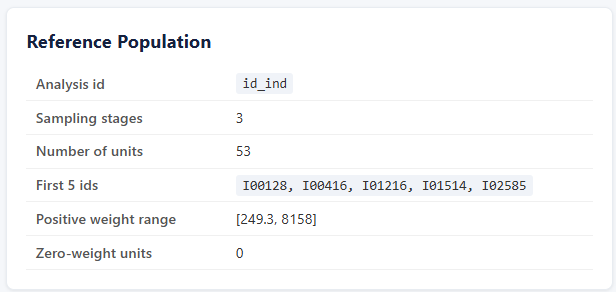
\includegraphics[width=1\linewidth]{figures/inspect_reference} \caption{Reference population card of the HTML report.}\label{fig:inspect-fig-reference}
\end{figure}

The first card describes the \textbf{reference population}: the set of
units, frozen at definition time, on which every estimation will be
based --- for a \texttt{qvar\_ms()} wrapper, the disseminated units of
the last sampling stage, together with their dissemination weights. It
is best read as the \emph{contract} between the wrapper and any
estimation file: whatever \texttt{data.frame} is passed at estimation
time is matched against these identifiers (extra rows are discarded,
missing units count as zeros, and a differently ordered file is silently
reordered --- the warnings discussed earlier in this vignette all
originate from this matching step). The card reports the analysis
identifier (the column the estimation file must contain), the number of
reference units, a preview of the first identifiers and weights, the
range of the positive weights and the number of zero-weight units.

\subsection{Per-stage cards}\label{per-stage-cards}

\begin{figure}
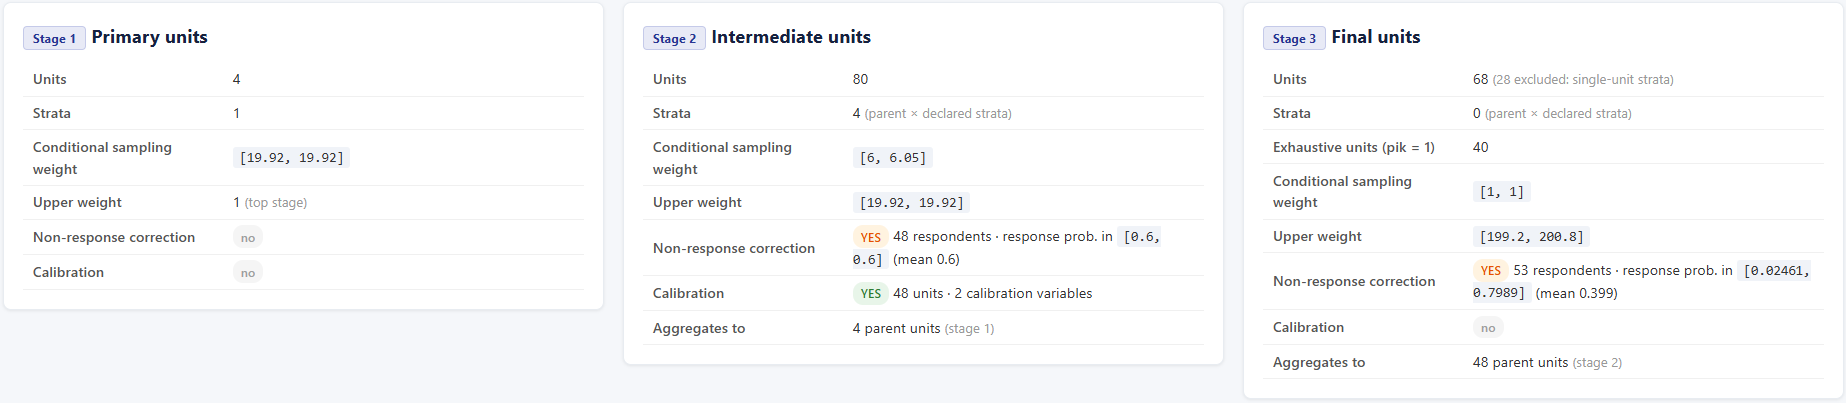
\includegraphics[width=1\linewidth]{figures/inspect_stages} \caption{Per-stage cards of the HTML report.}\label{fig:inspect-fig-stages}
\end{figure}

Each stage card summarizes what \texttt{qvar\_ms()} retained from the
declaration: number of sampled units and excluded units (single-unit
strata), number of effective strata (with the parent-crossing note from
stage 2 onwards), range of the conditional sampling weights and of the
cumulated Rao weight, non-response correction (with the range of the
estimated response probabilities) and calibration. These are computed
from the \emph{actual} technical data of the wrapper, not from the
arguments of the call --- which makes them a plausibility check as much
as a description. Two examples of what to look for, both drawn from real
debugging sessions:

\begin{itemize}
\tightlist
\item
  \textbf{response probabilities outside a plausible range} --- a
  \texttt{response\ prob.\ in\ {[}0.07,\ 0.12{]}} where the survey
  documentation says the response rate is around 70 \% is the signature
  of a \emph{cumulated} non-response weight declared where a
  \emph{conditional} one is expected (see the Conventions section); the
  estimation would run and silently inflate every variance component;
\item
  \textbf{an Upper (Rao) weight different from 1 at stage 1}, or a
  conditional weight range at odds with the sampling fractions of the
  design, points to the same family of weight convention errors.
\end{itemize}

\subsection{Methodological notes}\label{methodological-notes}

\begin{figure}
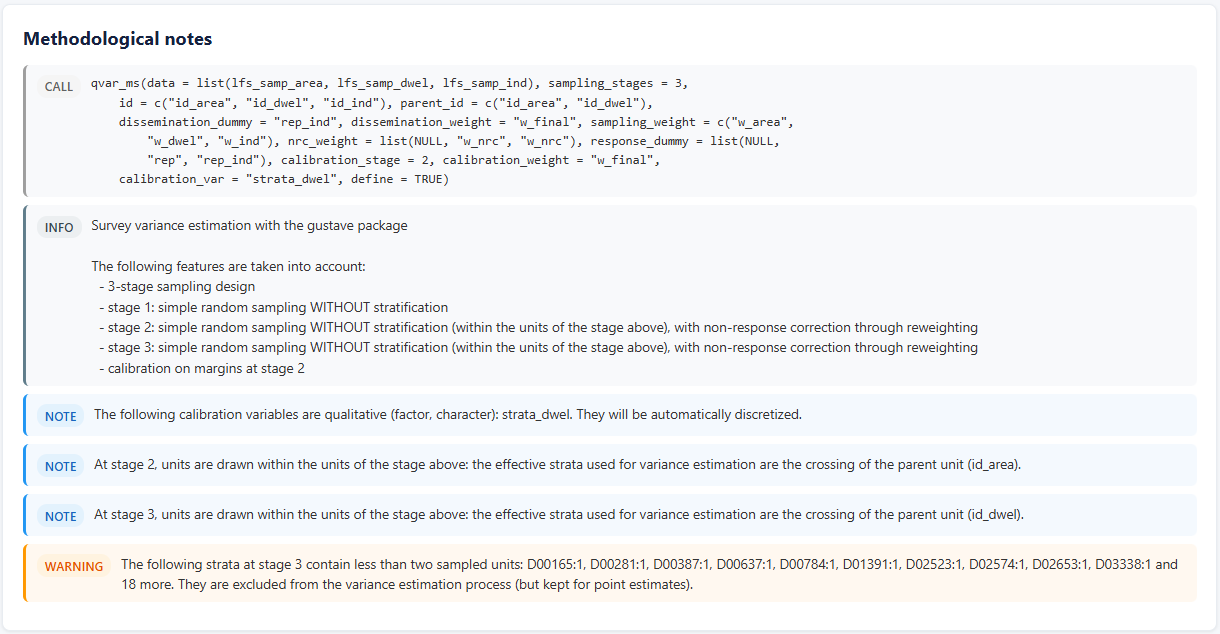
\includegraphics[width=1\linewidth]{figures/inspect_notes} \caption{Methodological notes card: notes and warnings emitted at definition time.}\label{fig:inspect-fig-log}
\end{figure}

The Methodological notes card replays, colour-coded, everything that was
printed when the wrapper was defined: the definition call itself, the
welcome message (INFO), the automatic coercions and strata-crossing
notes (NOTE, blue), and the warnings (orange) --- excluded single-unit
strata, unequal weights replaced by stratum means, suspicious
calibration g-ratios.

\subsection{Pipeline table and
diagram}\label{pipeline-table-and-diagram}

\begin{figure}
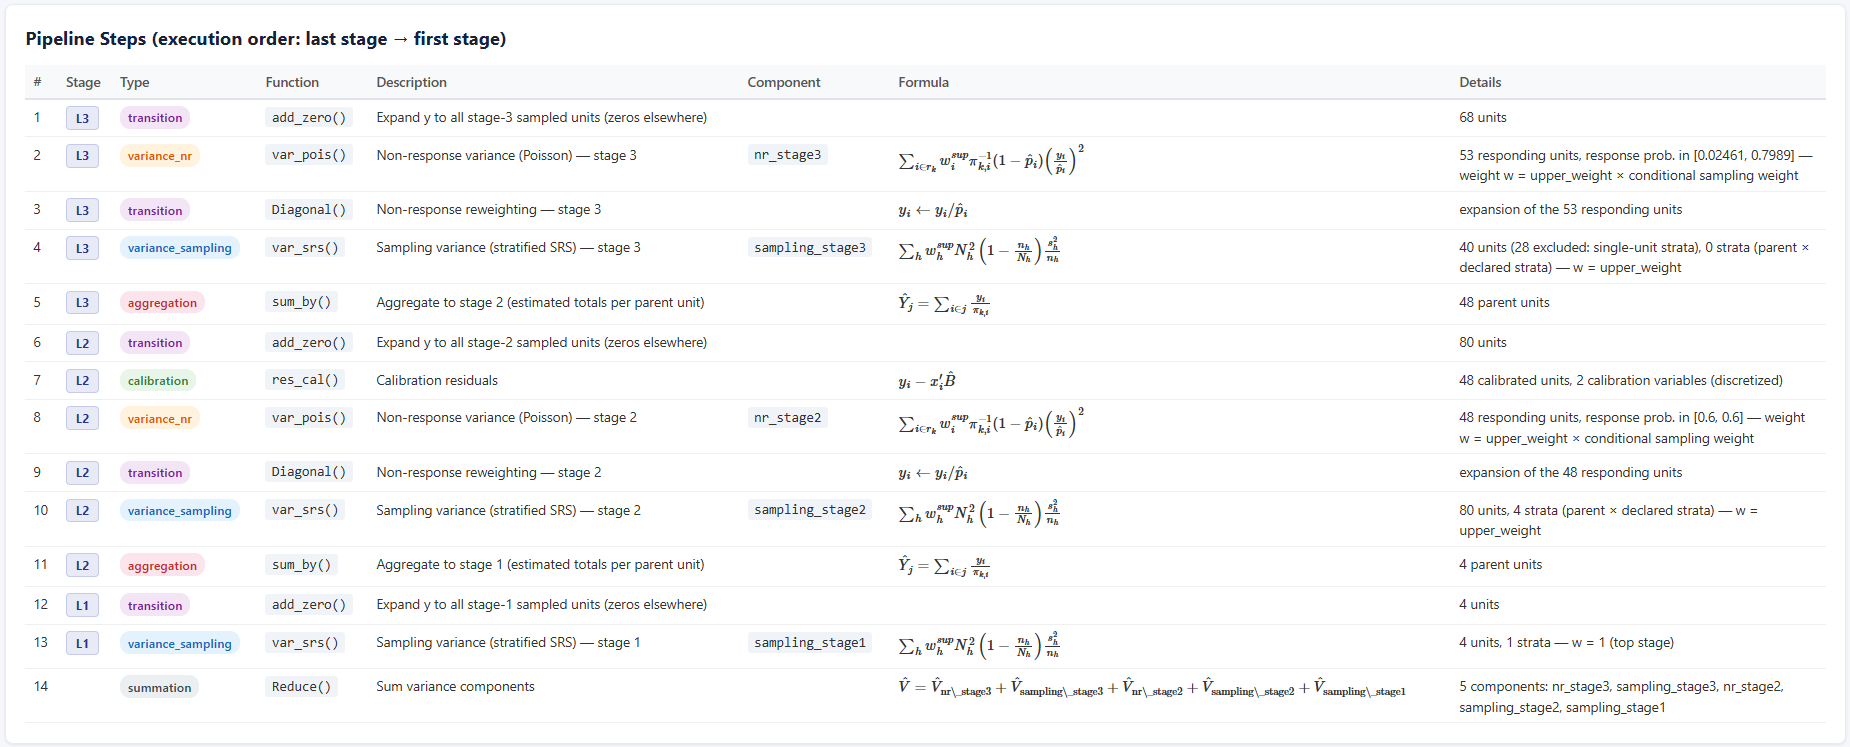
\includegraphics[width=1\linewidth]{figures/inspect_pipeline} \caption{The variance estimation pipeline}\label{fig:inspect-fig-pipeline}
\end{figure}

This is the heart of the report. One essential design decision deserves
a word: the pipeline is derived from the \textbf{technical data} of the
wrapper, not from the code of the variance function. The code is a
static loop with conditional blocks --- \texttt{res\_cal} and
\texttt{var\_pois} appear in it whether or not they will run, and
\texttt{var\_srs} appears once although it runs once \emph{per stage}.
What determines the actual execution is the content of
\texttt{technical\_data}: the inspector therefore rebuilds the pipeline
from it, so that the diagram shows exactly the steps that will execute,
stage by stage --- a calibration node only in the calibration stage's
subgraph, a non-response node only at corrected stages, one sampling
variance node per stage.

Each variance node carries the name of its component
(\texttt{nr\_stage2}, \texttt{sampling\_stage1}, \ldots). These names
are the same as those printed by the
\texttt{diagnostics\ =\ "components"} output and stored in the variance
list: the diagram is thus a legend for the numerical decomposition ---
when a component dominates, the diagram shows where in the design it
comes from.

\begin{figure}
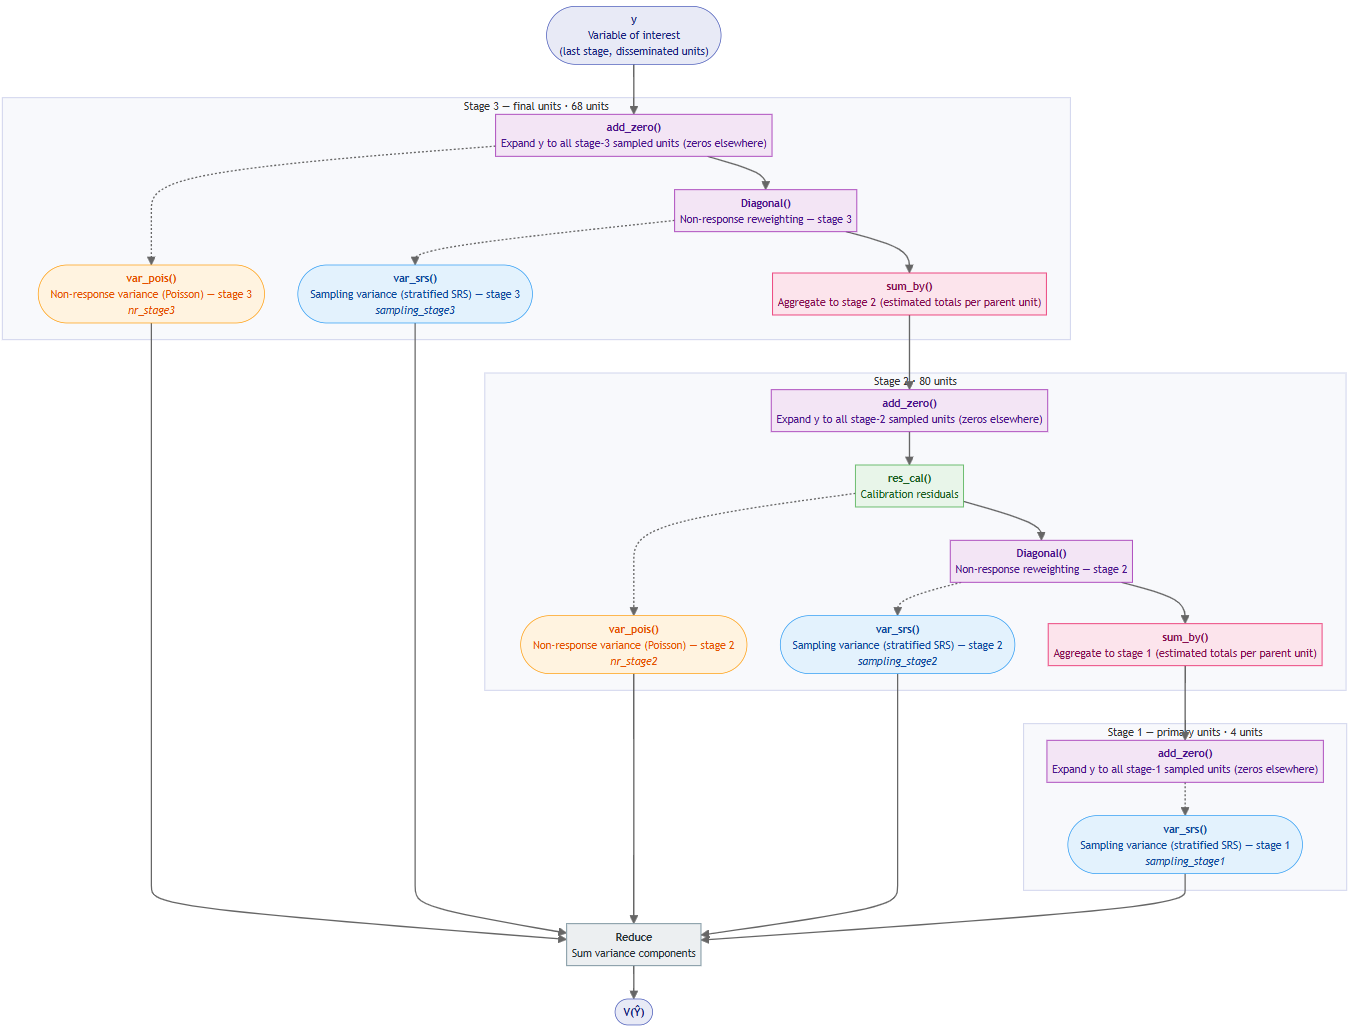
\includegraphics[width=1\linewidth]{figures/inspect_diagram} \caption{The variance estimation diagram}\label{fig:inspect-fig-diagram}
\end{figure}

\subsection{Technical parameters and raw technical
data}\label{technical-parameters-and-raw-technical-data}

\begin{figure}
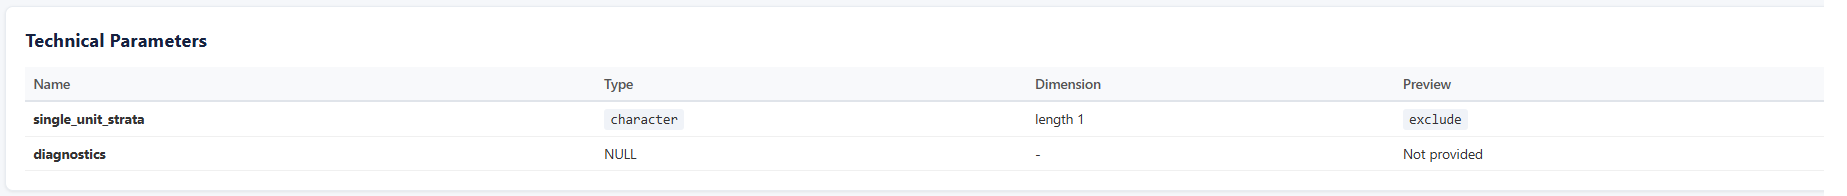
\includegraphics[width=1\linewidth]{figures/inspect_param} \caption{Technical parameters.}\label{fig:inspect-fig-param}
\end{figure}

The technical parameters cards lists the switchable arguments of the
wrapper (\texttt{single\_unit\_strata}, \texttt{diagnostics}) with their
defaults --- the knobs a user can turn at estimation time without
redefining anything.

\begin{figure}
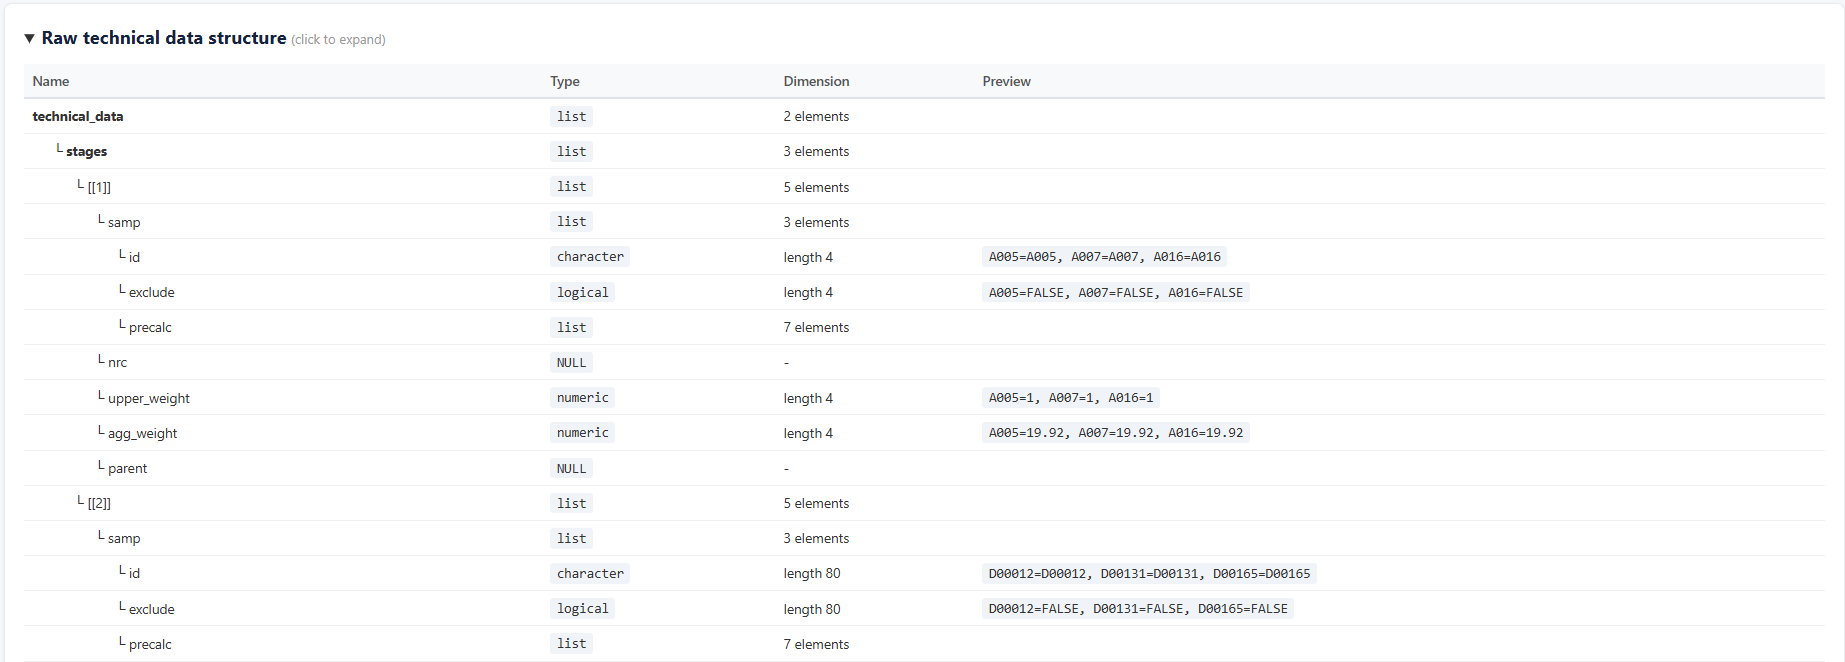
\includegraphics[width=1\linewidth]{figures/inspect_raw} \caption{Raw technical data.}\label{fig:inspect-fig-raw}
\end{figure}

The last card is a collapsible tree of the raw technical data,
descending recursively into the per-stage lists (identifiers, weights,
exclusion flags, precalculated matrices) with types, dimensions and
value previews. It is the map for advanced users who want to go beyond
the report.

Combined with \texttt{qvar\_notes()} for the methodological notes and
the \texttt{diagnostics} technical parameter for estimation-time output,
the inspector completes a three-level tooling: the \emph{log} tells what
happened at definition, the \emph{report} describes what the wrapper is,
and the \emph{diagnostics} tell what each estimation does.

\section{Conclusion}\label{conclusion}

This vignette started from a simple observation: \texttt{qvar()} made
analytical variance estimation accessible for the most common
single-stage case, but the surveys we actually run --- and the SAS
Poulpe programs we are migrating from --- are multistage.
\texttt{qvar\_ms()} extends the \texttt{qvar()} philosophy rather than
replacing it: the same declarative interface (one argument per
methodological feature), the same technical and methodological checks,
the same welcome message, and full backward compatibility, since a
single-stage call reproduces \texttt{qvar()} exactly (case 1). What
changes is the reach: an arbitrary number of sampling stages,
non-response correction at any subset of stages (declared through
response probabilities or conditional weights), calibration at any
stage, stratification crossed with the parent units, and a choice of
treatments for single-unit strata. The nine cases of this vignette
walked through this space one feature at a time, each validated against
a hand-built \texttt{define\_variance\_wrapper()} benchmark that makes
the underlying Rao (1975) decomposition explicit --- the same estimator
as the SAS Poulpe macros, which remain the external reference
throughout.

Along the way, the wrapper grew from a computing object into a
methodological one. The \texttt{diagnostics} technical parameter allows
a quality control of the variance estimation procedure --- variance
components with the exact effect of calibration, design effect and its
Kish decomposition, degrees of freedom, non-response and domain
diagnostics --- while \texttt{qvar\_notes()} and
\texttt{inspect\_wrapper()} make the wrapper itself readable: what
happened at definition time, what the encoded design is, and which
pipeline will actually execute.

More complex multistage cases --- unequal probabilities within strata,
balanced sampling at the first stage, shared or integrated weights ---
are to be handled with the core functions of the \texttt{gustave}
package, i.e.~\texttt{define\_variance\_wrapper()} together with
\texttt{varDT()}, \texttt{var\_pois()} and \texttt{res\_cal()},
following the patterns of the hand-built wrappers of this vignette.

Two directions naturally extend this work. The first is external
cross-validation against the \texttt{survey} package (Lumley, 2004), the
\emph{de facto} standard of the R ecosystem. Its default estimator for
multistage designs is the ultimate cluster approximation --- collapsing
all stages into a with-replacement sampling of primary units --- which
differs from the stage-by-stage Rao decomposition implemented here:
agreement is expected to be close but not exact, and the size and sign
of the differences (driven by the first-stage sampling fractions) would
be instructive in itself. A future section comparing \texttt{qvar\_ms()}
wrappers with the corresponding \texttt{svydesign()} objects, including
their respective treatments of lonely PSUs, would give users a second,
independent reference point next to \texttt{Poulpe}.

The second direction is downstream integration. A \texttt{gustave}
wrapper cleanly separates the design description from the data, which is
powerful for estimation but leaves the pairing of the two to the user.
Bundling them into a design object --- in the spirit of
\texttt{survey::svydesign()}, carrying the survey file together with its
variance wrapper --- would allow \texttt{gustave} to plug into the
growing ecosystem of tools built on such objects, notably
\texttt{fonctionr}, a package developed in Belgium that produces
publication-ready weighted analyses and visualizations from survey
design objects. Precision estimates would then flow directly into graphs
and tables, instead of living in a separate results file. This
design-object layer is under construction and beyond the scope of this
vignette.

\section{Annexe}\label{annexe}

\subsection{One responding unit: the Poisson term as the natural
continuation of the SRS
formula}\label{one-responding-unit-the-poisson-term-as-the-natural-continuation-of-the-srs-formula}

Two situations must be distinguished in a stratum. When it contains a
single \emph{sampled} unit, the SRS variance formula is undefined (the
\(s^2\) term divides by \(n - 1 = 0\)): this is the case handled by the
\texttt{single\_unit\_strata} treatment. When it contains several
sampled units of which a single one \emph{responds}, the SRS formula
remains perfectly defined, provided the non-responding units are kept in
the computation with a zero value --- which is exactly what the
\texttt{add\_zero()} mechanism of \texttt{gustave} does. This appendix
shows that, in the latter case, the SRS formula over all \(n\) sampled
units is \textbf{algebraically identical} to the Poisson variance term
of the lone respondent. This identity both explains why strata with a
single respondent require no special treatment, and motivates the
Poisson fallback as the natural continuation of the SRS formula when
even the zeros disappear. Notations follow Chauvet's lecture notes on
variance estimation (Ensai):
\url{https://ensai.fr/wp-content/uploads/2019/06/TechEchMaster_EstVariance_v1.pdf}

\subsubsection{From the Horvitz-Thompson variance
estimator}\label{from-the-horvitz-thompson-variance-estimator}

Under an arbitrary design, the total is estimated by \[
\hat t_{y\pi} = \sum_{k \in S} \frac{y_k}{\pi_k},
\] and its variance is estimated (without bias, provided all joint
inclusion probabilities are positive) by \[
\hat v_{HT}(\hat t_{y\pi}) = \sum_{k,l \in S}
\frac{y_k}{\pi_k} \frac{y_l}{\pi_l}
\frac{\pi_{kl} - \pi_k \pi_l}{\pi_{kl}}.
\] Suppose a single unit \(k\) of the sample carries a non-zero value
--- say, one respondent with \(y_k = 10\) among four units sampled with
\(\pi = 0.25\), the three non-respondents entering with \(y = 0\). Every
term of the double sum contains a product \(y_k y_l\) and therefore
vanishes, except the diagonal term \(k = l\). With the convention
\(\pi_{kk} = \pi_k\), the estimator collapses to \[
\hat v_{HT}(\hat t_{y\pi})
= \left(\frac{y_k}{\pi_k}\right)^2 \frac{\pi_k - \pi_k^2}{\pi_k}
= \left(\frac{y_k}{\pi_k}\right)^2 (1 - \pi_k),
\] which is precisely the contribution of unit \(k\) under a Poisson
design --- the term computed by \texttt{var\_pois()}.

\subsubsection{From the SRS formula with zeroed
non-respondents}\label{from-the-srs-formula-with-zeroed-non-respondents}

Under simple random sampling (equal inclusion probabilities
\(\pi_k = n/N\)), the total is estimated by \(\hat t_{y\pi} = N \bar y\)
with \(\bar y = \frac{1}{n} \sum_{k \in S} y_k\), and its variance by
the classical formula \[
\hat v(\hat t_{y\pi}) = N^2 \, \frac{1-f}{n} \, s^2_y,
\qquad
s^2_y = \frac{1}{n-1} \sum_{k \in S} (y_k - \bar y)^2,
\qquad f = \frac{n}{N}.
\] With a single non-zero unit \(k\), the sum of squares splits into the
contribution of the respondent and that of the \(n - 1\) zero-valued
units, each equal to \(\bar y^2\): \[
s^2_y = \frac{1}{n-1} \left( (y_k - \bar y)^2 + (n-1)\,\bar y^2 \right)
      = \frac{1}{n-1} \left( y_k^2 - 2 y_k \bar y + n \bar y^2 \right).
\] Since \(\bar y = y_k / n\), \[
s^2_y = \frac{1}{n-1}
\left( y_k^2 - \frac{2 y_k^2}{n} + \frac{y_k^2}{n} \right)
= \frac{y_k^2}{n-1} \cdot \frac{n-1}{n}
= \frac{y_k^2}{n}.
\] Injecting into the full formula, with \(f = \pi_k = n/N\): \[
\hat v(\hat t_{y\pi})
= N^2 \, \frac{1 - f}{n} \, \frac{y_k^2}{n}
= \left(1 - \pi_k\right) \frac{N^2 y_k^2}{n^2}
= \left(\frac{y_k}{\pi_k}\right)^2 (1 - \pi_k)
= \hat v_{HT}(\hat t_{y\pi}).
\]

\subsubsection{\texorpdfstring{How to use it in \texttt{qvar\_ms()}
?}{How to use it in qvar\_ms() ?}}\label{how-to-use-it-in-qvar_ms}

The two computations are rigorously identical: since the Deville-Tillé
formula implemented by \texttt{varDT()} reduces exactly to the classical
SRS estimator under equal inclusion probabilities, the identity holds
for the actual \texttt{gustave} computation. Two consequences for
\texttt{qvar\_ms()}. First, strata with a single \emph{respondent} among
several sampled units require no special treatment: the SRS formula with
zeroed non-respondents already computes the right quantity. Second, when
the stratum contains a single \emph{sampled} unit, \(s^2_y\) is
undefined but the diagonal Horvitz-Thompson term
\((1-\pi_k)(y_k/\pi_k)^2\) remains available: this is the term added by
\texttt{single\_unit\_strata\ =\ "poisson"}.

\section{References}\label{references}

\begin{itemize}
\tightlist
\item
  Caron N. (1998), ``Le logiciel Poulpe : aspects méthodologiques'',
  \emph{Actes des Journées de méthodologie statistique},
  \url{http://jms-insee.fr/jms1998s03_1/}
\item
  Chauvet G., Estimation de variance, \emph{Ensai},
  \url{https://ensai.fr/wp-content/uploads/2019/06/TechEchMaster_EstVariance_v1.pdf}
\item
  Kish L. (1965), \emph{Survey Sampling}, Wiley.
\item
  Kish L. (1992), ``Weighting for unequal P\_i'', \emph{Journal of
  Official Statistics}, 8(2), 183--200.
\item
  Little R.J.A., Vartivarian S. (2005), ``Does weighting for nonresponse
  increase the variance of survey means?'', \emph{Survey Methodology},
  31(2), 161--168.
\item
  Lumley T. (2004), ``Analysis of Complex Survey Samples'',
  \emph{Journal of Statistical Software}, 9(8), 1--19.
\item
  Rao J.N.K. (1975), ``Unbiased variance estimation for multistage
  designs'', \emph{Sankhya}, C n°37, 133--139.
\item
  Särndal C.-E., Lundström S. (2005), \emph{Estimation in Surveys with
  Nonresponse}, Wiley.
\item
  Särndal C.-E., Swensson B., Wretman J. (1992), \emph{Model Assisted
  Survey Sampling}, Springer.
\item
  Wolter K.M. (2007), \emph{Introduction to Variance Estimation}, 2nd
  ed., Springer.
\end{itemize}

\end{document}
